\documentclass[acmsmall,nonacm]{acmart}
\setcopyright{none}
\settopmatter{printacmref=false}
\renewcommand\footnotetextcopyrightpermission[1]{}
% Keep the complete affiliation under the title in this non-ACM manuscript.
\authorsaddresses{}
\makeatletter
\renewcommand{\department}[2][0]{#2\par\noindent}
\renewcommand{\institution}[1]{\global\@ACM@instpresenttrue#1\par\noindent}
% Geographic fields are intentionally omitted in this non-ACM author manuscript.
\renewcommand{\@ACM@checkaffil}{}
\patchcmd{\@typeset@author@line}{\unskip,}{\par\noindent}{}%
  {\ClassError{spatial-hls-survey}{Unable to format the author block}{Check the acmart author-line definition.}}
\makeatother
\usepackage{amsmath,mathtools,bm,booktabs,tabularx,listings,tikz}
\usepackage{xurl}
\setlength{\emergencystretch}{2em}
\renewcommand{\tabularxcolumn}[1]{>{\raggedright\arraybackslash}p{#1}}
\usetikzlibrary{arrows.meta,positioning,fit,calc}
\newcommand{\N}{\mathbb{N}}
\newcommand{\Z}{\mathbb{Z}}
\newcommand{\R}{\mathbb{R}}
\newcommand{\C}{\mathbb{C}}
\newcommand{\sem}[1]{\llbracket #1\rrbracket}
\newcommand{\pe}{\operatorname{pe}}
\newcommand{\pub}{\operatorname{pub}}
\newcommand{\rel}{\operatorname{rel}}
\newcommand{\hb}{\mathrel{\prec}}
\newtheorem{proposition}{Proposition}
\newtheorem{definition}{Definition}
\lstset{basicstyle=\small\ttfamily,columns=fullflexible,keepspaces=true,breaklines=true,frame=single,framerule=.3pt,numbers=left,numberstyle=\tiny,numbersep=6pt,showstringspaces=false,xleftmargin=1.4em}
\setlength{\headheight}{14pt}
\title[From Algorithm Semantics to Processing Elements]{From Algorithm Semantics to Processing Elements: A Survey of Spatial High-Level Synthesis}
\author{Lingzhi Yang}
\affiliation{\department{Applied Mathematics and Statistics}\institution{Stony Brook University}}
\date{September 10, 2026}
\begin{document}
\begin{abstract}
Compiling a mathematical algorithm for a spatial machine requires both constructing a useful distributed algorithm and realizing it on finite processing elements. This survey connects these two problems through recurrence equations, invariant-based algorithm derivation, communication localization, transform algebra, scheduling and bounded dataflow execution. Worked derivations follow a streaming filter from shared indices to local propagation, an FFT from factorization to inter-PE exchange, and a matrix product from reduction semantics to a communication protocol. QR, interval dynamic programming, sparse iteration and attention expose additional choices in state, topology and numerical behavior. Historical synthesis methods are compared with contemporary compiler infrastructures and concrete Cerebras CSL, AMD AI Engine and Tenstorrent interfaces. The resulting design synthesis treats algorithm alternatives, layout, timing and state as coupled search decisions, with explicit acceptance conditions at each refinement boundary. A companion Pragma prototype provides finite protocol checks and a bounded SDK-simulator experiment; it evaluates one part of the design rather than the proposed compiler as a whole.
\end{abstract}
\maketitle
\raggedbottom

\section{Introduction}
Spatial high-level synthesis (HLS) connects a mathematical operation to a program distributed across processing elements (PEs). There are two intertwined design problems. The first is constructive: discover a recurrence, factorization or traversal that exposes useful locality and parallelism. The second is realizational: assign that organization to finite processors, memories and communication resources while preserving its values and state transitions. A filter may replace shared reads with a propagation chain; a factorization may maintain a streaming triangular state or reduce block factors along a tree. These algorithm decisions precede, and constrain, instruction scheduling and routing.

Several mature traditions supply constructive methods. Invariant-based development derives the partial state an algorithm maintains. Systolic synthesis localizes communication and allocates recurrence dimensions to space and time. Transform generators search algebraic decompositions and implementation forms. Process networks and synchronous dataflow explain stream composition, rates and delayed state; polyhedral and modulo scheduling organize dependence and resource constraints. Modern HLS and extensible intermediate representations (IRs) provide engineering mechanisms for combining these methods. Their assumptions differ, so composition requires more than connecting graph-shaped interfaces.

Our organizing question is therefore: which representations let a compiler construct and compare spatial algorithms, and which facts must survive their realization as finite PE programs? We compare methods by their search objects, transformation mechanisms, applicable problem classes and unresolved implementation choices. The distinction between mathematical equivalence and machine behavior remains central: a useful decomposition may still exceed local storage, alter floating-point behavior or create incompatible stream orders. Conversely, a perfectly checked implementation can embody a poor algorithmic choice.

Sections~\ref{sec:scope}--\ref{sec:semantics} establish scope and semantics; Section~\ref{sec:constructive} develops constructive methods. Scheduling, transform generation and compiler representations lead to worked examples, backend interfaces and the workload synthesis in Section~\ref{sec:applications}. Section~\ref{sec:design} proposes a research design. The appendices delimit source-reading scope and the Pragma companion's finite checks. That experiment covers an existing SUMMA backend, not the full proposed compiler.



\section{Scope and Historical Distinctions}\label{sec:scope}
\subsection{Selection and evidence}
The bibliography is a purposive technical selection covering algorithm construction, spatial organization and executable realization. Backward reference tracing and a targeted audit of a local systolic-algorithm library connect recent compilers to recurrence synthesis, program invariants, signal processing, numerical linear algebra and early programmable arrays. Works are retained when a representation, construction method or limitation changes an engineering decision. This is not an exhaustive systematic review or a complete history of parallel computing. The inspected corpus and section-level reading scopes are recorded in the companion notes. Primary papers establish historical claims; versioned source and official documentation establish inspected engineering behavior. Reported performance from incompatible devices or workloads is not combined into a ranking.

Four kinds of statements require different evidence. A literature result is attributed with its original assumptions. A derivation in this paper is stated mathematically and checked on a small executable example when useful. An implemented feature identifies its source and acceptance boundary. A measurement identifies its inputs, target and measurement interval. This separation is necessary because a syntactically valid IR, a numerically correct output and a live bounded runtime establish different properties.

\subsection{Dataflow has several meanings}
Flynn's taxonomy classifies organizations by instruction and data streams~\cite{flynn1972}; it does not classify the semantics of a graph language. MIMD describes independent instruction streams, while dataflow can describe either a dependency-based execution rule or a language whose processes communicate through streams. A MIMD machine may execute a statically planned systolic algorithm, and a sequential processor can interpret a dataflow graph. Dennis and Misunas' processor work makes operand-driven execution concrete~\cite{dennis1975}, whereas Kahn's process semantics gives a mathematical account of communicating sequential processes~\cite{kahn1974}. These are related questions at different abstraction levels.

Systolic design couples a recurrence to local communication and repeated computation~\cite{kung1982}. Its regularity can reduce global data movement, but a systolic array is one algorithmic organization rather than a synonym for every dataflow machine. The first TPU's matrix unit illustrates a specialized systolic datapath~\cite{jouppi2017}; an FPGA can instantiate a selected datapath, while a programmable spatial array runs local instruction streams on preexisting resources. The compiler decides different things in each case: hardware construction, configuration of a fixed fabric, or software scheduling on that fabric.

TensorFlow's graph representation, TVM's compilation pipeline and Triton's tiled kernel model expose useful but different program structure~\cite{abadi2016,chen2018tvm,tillet2019}. A tensor DAG edge commonly identifies a value or buffer dependence. It does not automatically specify a FIFO rate, a network route, a scratchpad lifetime or a state-reset protocol. That missing information can be supplied by lower-level compilation; it should not be silently attributed to the high-level graph.

CUDA offers a useful comparison point for GPU programmers. Its thread/block hierarchy and SIMT execution make locality, synchronization scope and occupancy central concerns. Current CUDA also provides thread-block clusters and distributed shared memory within a cluster~\cite{cuda2026}. Thus the engineering difference is not that GPUs lack explicit communication or local synchronization. For the spatial targets considered here, physical data distribution and resource allocation persist more directly in the generated program, and the compiler must supply the local communication protocol required by the chosen backend. Neither architectural style eliminates data movement or synchronization costs.

\begin{figure}[t]
\centering
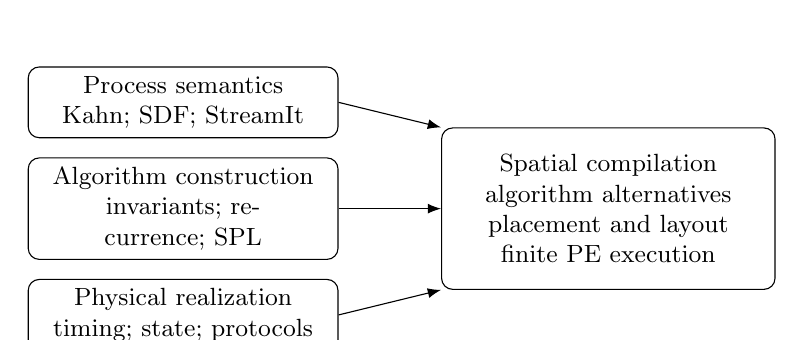
\begin{tikzpicture}[font=\small,box/.style={draw,rounded corners,align=center,text width=3.7cm,minimum height=.8cm},>=Latex]
\node[box] (sem) at (0,2.7) {Process semantics\\Kahn; SDF; StreamIt};
\node[box] (map) at (0,1.35) {Algorithm construction\\invariants; recurrence; SPL};
\node[box] (hw) at (0,0) {Physical realization\\timing; state; protocols};
\node[box,text width=4cm,minimum height=2.05cm] (compiler) at (5.4,1.35) {Spatial compilation\\\small algorithm alternatives\\placement and layout\\finite PE execution};
\draw[->] (sem.east) -- (compiler.north west);
\draw[->] (map.east) -- (compiler.west);
\draw[->] (hw.east) -- (compiler.south west);
\end{tikzpicture}
\caption{Three bodies of knowledge meet in spatial compilation. The arrows indicate conceptual requirements, not a claim that the cited systems form a single historical lineage.}
\Description{Three boxes for process semantics, spatial algorithm structure, and implementation semantics feed a box for spatial compilation.}
\label{fig:background}
\end{figure}

\section{What Must Be Preserved}\label{sec:semantics}
\subsection{Values, effects and persistent state}
A useful source contract includes more than a function signature. For a stateless operation, $f:X\to Y$ specifies mathematical values. For a recurrent operation, use a state transition
\begin{equation}
 (s_{t+1},y_t)=F(s_t,x_t),\qquad s_0=\operatorname{init}(\eta),
\end{equation}
where $\eta$ identifies the instance or request. A contract must define whether reset discards state, whether updates can overlap, and which effects are externally observable. Sharing immutable weights between instances is different from sharing a mutable accumulator or KV-cache entry. An effect graph should order conflicting reads/writes and host-visible actions even when their tensor shapes are unrelated.

The mathematical domain and the machine domain must also be separated. An algebraic real-valued map, an IEEE floating-point program with a fixed evaluation order, and a fixed-point implementation with saturating arithmetic are different specifications. Layout is another independent component: a tensor coordinate can map to a PE, memory bank, address and vector lane. Moving or reinterpreting those coordinates must preserve both values and the consumer's access contract.

\subsection{Streams and fixed points}
Let $\mathcal S(V)$ contain finite and infinite streams over a token domain $V$, ordered by prefix. A process is a continuous function on a product of these domains. For fixed external input $I$, the equations $X=F(X,I)$ have a least-fixed-point interpretation obtained from increasing finite approximations~\cite{kahn1974,leeparks1995}:
\begin{equation}
 X^*=\bigsqcup_{n\ge0} F_I^n(\bot).
\end{equation}
Continuity means finite output information depends on finite input information; it is a condition on the stream function, not a hardware timing promise. Deterministic processes with blocking reads and unbounded nonblocking writes provide a powerful compositional model. A merge that chooses whichever input arrives first requires a different determinacy argument. Similarly, bounded writes add observable blocking behavior that is absent from the unbounded model.

The distinction between an actor language and a coordination language is useful in compiler construction. A local kernel can be written in C++, CSL or another imperative language, while its firing conditions and communication belong to a surrounding network language. StreamIt's structured stream composition supplies an example of a restricted coordination model designed to support analysis and optimization~\cite{thies2002}. Restricting the coordination language can be more valuable than pretending to analyze arbitrary local code.

Geilen and Basten identify a stronger operational requirement than merely avoiding global deadlock~\cite{geilen2003}. A bounded implementation can leave one component permanently blocked while another continues producing output. Their scheduler detects local artificial deadlocks through chains of waiting processes and increases the smallest full FIFO on each deadlock by a finite amount. Their completeness and boundedness result assumes a bounded, effective KPN: fairness and maximality are evaluated against the corresponding unbounded network, and internal tokens are eventually consumed. Merely scheduling the bounded implementation's enabled transitions fairly is insufficient. The paper separately discusses undecidability of boundedness/effectiveness and impossibility results for broader scheduling classes. Its positive theorem does not supply a compile-time capacity bound for a fixed wafer. Possible engineering responses include restricted coordination languages, resource annotations, or runtimes able to reject or migrate work when physical capacity is exhausted.

\subsection{Rates, markings and finite storage}\label{sec:rates}
For a synchronous dataflow graph, let channel $e:u\to v$ produce $p_e$ tokens per firing of $u$ and consume $c_e$ per firing of $v$. A periodic execution with repetition counts $q_u,q_v$ requires
\begin{equation}\label{eq:balance}
 p_eq_u-c_eq_v=0\quad\text{for every }e,
 \qquad\text{or}\qquad \Gamma q=0,\ q>0.
\end{equation}
Fixed rates permit static scheduling~\cite{lee1987static}. They do not make the initial marking irrelevant: a cycle of actors that each needs an input token and has no initial token is consistent but cannot start.

To account for finite storage, distinguish completed publications $P_e(t)$ from completed reclamations $R_e(t)$. If tokens occupy equal-sized slots, the number of occupied or retained slots is
\begin{equation}\label{eq:occupancy}
 O_e(t)=m_e^0+P_e(t)-R_e(t).
\end{equation}
If $W_e(t)$ slots are reserved for unfinished writes, capacity requires
\begin{equation}\label{eq:capacity}
 0\le O_e(t)+W_e(t)\le B_e.
\end{equation}
A logical read need not reclaim its slot: a consumer or DMA engine may still be using it. Credit return must therefore refer to the relevant physical lifetime. Equation~\eqref{eq:occupancy} alone cannot determine which operations are enabled.

Stuijk, Geilen and Basten formalize timed CSDF with firing-start, firing-end and clock transitions, including possible auto-concurrency~\cite{stuijk2008}. Reverse channels encode storage credits. In their chosen abstraction, an actor reserves its output space at start and returns its input space at end. This provides a conservative abstraction when an implementation reserves later or releases earlier under the paper's stated timing conditions. Their throughput-buffer exploration concerns that model; it does not assign shared functional units or analyze arbitrary imperative memory accesses automatically.

\subsection{Trace refinement and progress}
Let $T$ be the target transition system, $S$ the source semantics, and $\alpha$ erase target-internal events while reconstructing source-level observations. A safety claim can be expressed as
\begin{equation}
 \alpha(\operatorname{Traces}(T))\subseteq\operatorname{Traces}(S).
\end{equation}
For deterministic finite computations, the numerical observation relation may instead permit a stated error bound. Trace inclusion alone admits an implementation that stops forever after a valid prefix. A progress obligation must additionally state admissible environments, fairness, resource availability and termination or productivity requirements. These are separate obligations, even if one checker reports both for a restricted model.

Latency-insensitive design supplies a strong precedent: under its stallability and patient-process assumptions, adding stalls can preserve the ordered informative events while changing their timing~\cite{carloni2001}. An arbitrary task with side effects, a timeout, or an externally visible reset cannot be assumed to satisfy those hypotheses. The correct lesson is to identify a refinement-compatible interface, then prove that the implementation inhabits it.



\section{Constructing Spatial Algorithms}\label{sec:constructive}
Spatial synthesis begins before a placement function is chosen. A mathematical operation can admit different recurrences, factorizations, intermediate states and communication organizations. Three constructive questions recur in the literature: which partial results should be maintained, how should shared values move between their uses, and which dimensions should represent processors or time? Treating a source loop nest as the only algorithm loses these choices before physical optimization starts.

\subsection{Invariants select algorithms, not only proofs}
Chandy and Misra derive systolic programs from invariants~\cite{chandy1986}. Their program executes one simultaneous multiple assignment repeatedly: every right-hand side reads the preceding state. This gives precise meaning to a picture in which every cell updates at once. Invariants indexed by the logical step determine dataflow rates, initial values and boundary behavior during construction. The paper deliberately defers many physical-realization constraints. Its contribution is therefore complementary to geometric synthesis: a space--time diagram can be derived from an invariant-maintaining program instead of being the object from which correctness is guessed.

FLAME provides a related method at matrix-algebra granularity~\cite{gunnels2001}. Partitioning the postcondition $A=LU$ yields
\begin{equation}\label{eq:block-lu}
\begin{aligned}
 A_{11}&=L_{11}U_{11}, & A_{12}&=L_{11}U_{12},\\
 A_{21}&=L_{21}U_{11}, & A_{22}&=L_{21}U_{12}+L_{22}U_{22}.
\end{aligned}
\end{equation}
Here the leading block grows as the algorithm advances; $L$ is unit lower triangular. For an unpivoted construction, the required pivots or leading blocks must be nonsingular. Nonsingularity of the full matrix alone is insufficient. Selecting which equalities or partial updates already hold at a loop boundary selects the invariant and helps derive the next update. The original paper develops five useful invariants under its stated monotone-progress assumptions; it does not claim to enumerate all algorithms.

For example, once the leading factors and off-diagonal panels exist, a right-looking realization maintains the trailing Schur complement
\begin{equation}
 S_{22}=A_{22}-L_{21}U_{12}.
\end{equation}
A left-looking realization delays updates to a panel until that panel is needed. This changes the organization of reuse, reductions and live intermediates even though both compute the same exact unpivoted factorization when defined. On a spatial machine, immediate trailing updates may expose many resident output tiles; delayed panel updates may reduce the active frontier while requiring earlier factors to remain available. These are workload- and placement-dependent tradeoffs, not a universal performance ordering. A compiler capable only of permuting loops after a single invariant has been chosen explores a narrower space than a generator capable of changing the invariant itself.

\subsection{From a shared read to a local propagation}
A repeated expression can reveal communication opportunities. Suppose iteration point $z$ reads $x(h(z))$, with $h(z)=Az+b$. If an integer vector $u$ satisfies $Au=0$, then
\begin{equation}\label{eq:reuse-kernel}
 h(z-u)=h(z).
\end{equation}
Thus uses separated by $u$ require the same value. On a finite domain $D$, one possible localization introduces
\begin{equation}\label{eq:localize}
 X(z)=
 \begin{cases}
 X(z-u),&z-u\in D,\\
 x(h(z)),&z-u\notin D.
 \end{cases}
\end{equation}
This elementary construction is correct when every predecessor chain reaches the boundary and the boundary read is defined. A strictly decreasing integer height on each chain is a sufficient termination argument. It replaces repeated reads by boundary injection and forwarding; it also creates storage, latency and routing obligations.

Dezan et al.'s Alpha du Centaur system incorporates equation reindexing, communication localization, I/O pipelining and control generation in a trajectory toward circuit descriptions~\cite{dezan1991}. Localization is therefore an established synthesis transformation, not a new consequence of modern graph IRs. Their method also separates an index transformation from its effect on all occurrences and domains. Inputs and outputs may need extended domains to reach boundary cells; conditions dependent on time require generated control streams, while conditions fixed by PE coordinates can specialize cell behavior.

The nullspace observation is useful but does not solve every broadcast problem. Wong and Delosme study regular affine dependence algorithms whose dependence linear parts are either identity maps or rank-deficient broadcast maps~\cite{wong1992}. Their general propagation construction uses a unimodular basis and conditional propagation directions; a single simple nullspace-based localization need not suffice. More decisively, eliminating a broadcast is not the same optimization problem as obtaining an efficient systolic array. Basis selection affects propagation length, the number of propagated variables, geometric locality and dependence cycles across the whole algorithm. Their search bounds basis entries, considers inverse-basis costs and rejects unsuitable combinations of cycle displacements. The constructive lesson is to search communication forms together with schedules and geometry, rather than promise that each shared read independently becomes a cheap nearest-neighbor transfer.

\subsection{Worked derivation: a streaming FIR filter}
Consider a causal length-$K$ filter with resident coefficients, $K\ge1$, producing exactly $N\ge1$ outputs indexed by $0\le n<N$:
\begin{equation}\label{eq:fir}
 y_n=\sum_{k=0}^{K-1}h_kx_{n-k},\qquad x_n=0\ \text{for }n<0.
\end{equation}
We derive one spatial organization to make the preceding choices explicit. The shared-input map is $h_{\mathrm{in}}(n,k)=n-k$, whose integer kernel contains $(1,1)$. Introduce
\begin{equation}\label{eq:fir-local}
\begin{aligned}
 X(n,0)&=x_n, & X(n,k)&=X(n-1,k-1)\quad(k>0),\\
 C(n,-1)&=0, & C(n,k)&=C(n,k-1)+h_kX(n,k).
\end{aligned}
\end{equation}
Set $X(n,k)=0$ for negative $n$ as startup state. Induction gives $X(n,k)=x_{n-k}$ and $C(n,k)=\sum_{j=0}^{k}h_jx_{n-j}$; hence $y_n=C(n,K-1)$. This derivation preserves an explicit ascending accumulation order. It does not use associativity to replace the sum by a different reduction tree.

Assign tap $k$ to PE $k$ and seek a macro-operation issue schedule
\begin{equation}\label{eq:fir-schedule}
 \pi(n,k)=k,\qquad \theta(n,k)=an+bk.
\end{equation}
The input-forwarding dependence has schedule distance $a+b$; the accumulator dependence has distance $b$. If $d_X$ bounds the required forwarding delay and $d_C$ bounds the MAC-to-next-PE availability delay in the chosen profile, necessary ordering constraints are
\begin{equation}
 a+b\ge d_X,\qquad b\ge d_C.
\end{equation}
Successive outputs reuse a tap PE every $a$ time units, so its issue interval must also fit $a$. The two streams may contend for a physical link or queue; the inequalities alone do not allocate that resource. In an ideal profile with both availability bounds equal to one and independent stream resources, $a=b=1$ gives one-sample initiation, one-step partial-sum movement and two-step input movement. The unequal delays are part of the design, not an indexing accident.

\begin{figure}[ht]
\centering
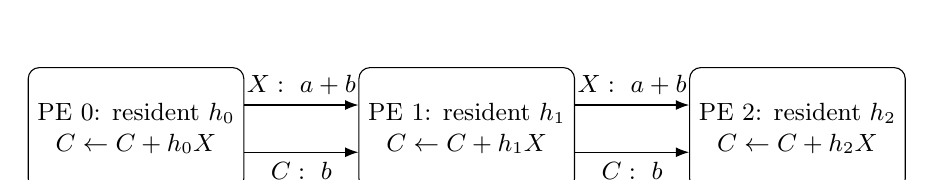
\begin{tikzpicture}[>=Latex,font=\small]
\foreach \k/\x in {0/0,1/4.2,2/8.4}{
 \node[draw,rounded corners,minimum width=2.7cm,minimum height=1.55cm,align=center] (p\k) at (\x,0) {PE $\k$: resident $h_{\k}$\\$C\leftarrow C+h_{\k}X$};
}
\draw[->] ([yshift=3mm]p0.east) -- node[above] {$X:\ a+b$} ([yshift=3mm]p1.west);
\draw[->] ([yshift=-3mm]p0.east) -- node[below] {$C:\ b$} ([yshift=-3mm]p1.west);
\draw[->] ([yshift=3mm]p1.east) -- node[above] {$X:\ a+b$} ([yshift=3mm]p2.west);
\draw[->] ([yshift=-3mm]p1.east) -- node[below] {$C:\ b$} ([yshift=-3mm]p2.west);
\end{tikzpicture}
\caption{The first three taps of the derived FIR organization. Edge labels are logical schedule distances, not measured link latencies. The $X$ stream advances both the sample and tap indices; the $C$ stream advances only the tap index. Delays or queues align the two arrivals at each MAC.}
\Description{Three adjacent tap processors exchange an input stream with delay a plus b and an accumulator stream with delay b. Each processor holds one coefficient.}
\label{fig:fir}
\end{figure}

The local actor body can be expressed without committing to a backend API:

\begin{lstlisting}[float=htbp,caption={An illustrative ordered FIR tap; forwarding and release are separate actions.}]
for n in output_indices:
    x = input_stream.acquire(sample=n-k)
    c = zero_value() if k == 0 else partial_stream.acquire(output=n)
    z = ordered_mac(c.value, h[k], x.value)
    if k+1 < K and n+1 < N:
        forward_input(x.value, sample=n-k, next_output=n+1)
    publish_partial(z, output=n)
    release_after_last_use(x, c)
\end{lstlisting}

Here \texttt{output\_indices} is $0,\ldots,N-1$. Tap zero reads the $N$ host samples. Each downstream $X$ channel is initially seeded with the zero corresponding to $X(-1,k-1)$ at destination tap $k$; its $N-1$ forwarded values then supply outputs $1,\ldots,N-1$. Each partial-sum channel carries exactly $N$ values. The final tap publishes to the output interface. Suppressing the last input forwarding prevents an unconsumed token for nonexistent output $N$; computing a convolution tail would require a different output domain. For asynchronous forwarding, the last-use event includes transfer completion. A backend may replace physical startup-zero tokens with local initialization, provided it preserves this token accounting. The zero at tap zero is an immediate value and has no borrowed storage to release.

Folding this direct $K$-MAC-per-output realization onto $P<K$ single-issue MAC processors introduces a distinct throughput problem. Work conservation requires an average output interval of at least $K/P$ cycles; a constant integer initiation interval is therefore at least $\lceil K/P\rceil$. Nonuniform periodic intervals need only satisfy the average bound. Neither bound is a construction or a bound for every alternative filtering algorithm. A one-PE realization can scan all taps using a sample ring buffer, retaining coefficients and accepting samples at a slower rate. Its storage and memory-port requirements differ from the fully spatial chain. A useful source abstraction preserves the FIR equation while allowing both organizations to be generated and compared.

\subsection{Projection, offsets and retiming are different choices}
Rao and Kailath distinguish processor allocation from the schedule of a regular iterative algorithm~\cite{raokailath1988}. For a one-dimensional iteration direction $u$, a projection $P$ with kernel spanned by $u$ groups points on the same processor. A uniform affine schedule allows variable-specific offsets,
\begin{equation}
 s_x(z)=\ell^Tz+\gamma_x.
\end{equation}
If $y(z)$ depends on $x(z-d)$, their unit-step ordering constraint becomes
\begin{equation}\label{eq:ria-offset}
 \gamma_y-\gamma_x+\ell^Td\ge1.
\end{equation}
Offsets allow ordering between different variables at the same index point, where a common purely linear schedule fails. The condition $\ell^Tu\ne0$ separates successive instances of one variable assigned to the same processor. Their global-step model permits at most one computation of each indexed variable per processor per step; it is not a single-instruction-per-cycle machine model. Variable kinds still need local scheduling on a programmable PE. Likewise, changing the basis of the projection's row space preserves the grouping but can change edge geometry in physical coordinates.

Retiming acts on an already constructed synchronous network rather than selecting its recurrence. In Leiserson and Saxe's graph model, vertices have combinational delays and edge $e:u\to v$ contains $w(e)$ registers~\cite{leiserson1991}. An integer lag assignment gives
\begin{equation}\label{eq:retime}
 w_r(e)=w(e)+r(v)-r(u).
\end{equation}
Nonnegative edge counts are required. Cycle register totals remain invariant by telescoping, so a legal retiming can redistribute delay and reduce the longest combinational path without inventing extra delay around a recurrence cycle. This is a precise optimization space, distinct from adding arbitrary FIFO capacity or changing an algorithm's iteration distance. For a software target, an analogous transformation must also preserve initial values, externally visible timing requirements and the meaning of stored tokens; register counts alone do not establish that adapter relation.

Together these methods suggest a richer search object than a scheduled operation DAG: an algorithm alternative, a localization of shared values, an allocation of iterations, and a representation of delayed state. The following section adds dependence and physical-resource constraints to that constructive space.


\section{Scheduling, Placement and Physical Feasibility}\label{sec:scheduling}
\subsection{Recurrence equations before a machine schedule}
Uniform recurrence equations describe families of computations with constant dependence displacements. Karp, Miller and Winograd separate a finite graph of equation kinds from its expansion over lattice points~\cite{kmw1967}. Their schedule orders evaluations after their predecessors; the free schedule assigns the earliest possible unit-time evaluation, without a fixed processor bound. Their existence results depend on the domain, including positive orthants, and on weighted dependence cycles. They are not a claim that every acyclic-looking equation graph fits a finite array: a self-edge in the equation graph can encode an ordinary time recurrence rather than a cycle between identical dynamic instances.

For example, consider the illustrative recurrence
\begin{equation}\label{eq:stencil}
 u(t,i)=a u(t-1,i-1)+b u(t-1,i)+c u(t-1,i+1)
\end{equation}
with specified initial values and boundary conditions. All three dependencies advance the logical time coordinate by one. Setting $\pi(t,i)=i$ and $\theta(t,i)=t$ respects the value ordering, but an implementation that uses a remote neighbor value must additionally accommodate transfer and arithmetic latency. Scaling $\theta$ or retiming the communication can address this under a chosen target profile. A declaration of independence between values at equal $t$ does not remove those implementation costs.

Alpha expresses variables over integer points of polyhedral domains and supports transformations from equations toward regular architectures~\cite{alpha1991}. This is an established language-level antecedent to high-level spatial synthesis. Unlike a trace of an already scheduled machine, an equational representation need not identify an index coordinate with physical time. Domain transformations, localization of communication and allocation of repeated values are distinct decisions.

Wilde's language report defines equivalence through agreement of domain, type and pointwise denotation~\cite{alpha1994}. Its affine dependence operator is especially instructive. For $h(z)=Az+b$ and expression $E$ defined over $D_E$,
\begin{equation}\label{eq:alpha-domain}
 (E\circ h)(z)=E(Az+b),\qquad D_{E\circ h}=h^{-1}(D_E).
\end{equation}
Composing $h$ with $g(z)=Cz+d$ yields $ACz+Ad+b$, but the domain must be transformed with it. A compiler that rewrites the address arithmetic and forgets the preimage can introduce out-of-domain reads. Alpha's reduction operator additionally assumes associative, commutative combination, and the report assumes unbounded arithmetic precision. These assumptions explain both its algebraic power and the need for a separate numerical contract when lowering to machine arithmetic.

\subsection{Affine dependence constraints}
For statement $S$, an iteration domain $D_S$ and an access relation identify the dynamic instances and their data dependences. A schedule assigns each instance an affine vector $\theta_S(i,p)$, where $p$ contains shape parameters. Dependence pairs $(S,i)\to(T,j)$ require lexicographic precedence:
\begin{equation}
 \theta_T(j,p)-\theta_S(i,p)\succ_{\mathrm{lex}}0.
\end{equation}
For one schedule dimension, nonnegativity over a rational dependence polyhedron can be reduced to linear constraints with affine Farkas multipliers. If $D=\{z:Az+b\ge0\}$ is nonempty, an affine expression $g(z)$ nonnegative on $D$ admits
\begin{equation}
 g(z)=\lambda_0+\lambda^T(Az+b),\qquad\lambda_0,\lambda\ge0.
\end{equation}
This is the rational-polyhedron statement. Replacing integer dependences with a relaxation can lose opportunities; it is not a universal equivalence for arbitrary sets of integer points. Multidimensional scheduling handles dependences not strictly ordered in the first dimension~\cite{feautrier1992a,feautrier1992b}. Vivien's analysis is especially useful for bounding ``optimal'' claims: minimal schedule dimension is established within a specified affine, per-statement framework, not for arbitrary schedules or physical-machine performance~\cite{vivien2002}.

A dependence relation may include flow, anti- and output dependences from aliased storage. Renaming or privatizing storage can remove the latter two only if the source effect and interface contracts permit it. A frontend that sees only operation names loses the information required to distinguish a legal schedule transformation from an invalid reorder.

\subsection{Resource constraints and initiation interval}
A schedule that orders values still needs an implementation schedule. Let $r$ be a resource with capacity $C_r$, and let operation $o$ occupy it over an interval $I_{o,r}$. A direct feasibility condition is
\begin{equation}\label{eq:resource}
 \sum_o \mathbf1\{t\in I_{o,r}\}\le C_r\qquad\text{for every }r,t.
\end{equation}
The interval represents occupancy rather than necessarily the full result latency. A pipelined multiplier may accept a new independent operation every cycle while an accumulator recurrence waits several cycles for its previous value. Conflating latency with initiation interval hides both missed parallelism and illegal dependencies.

For modulo scheduling, a dependence cycle with total latency $\ell$ and positive total iteration distance $d$ requires $\mathrm{II}\ge\lceil\ell/d\rceil$. A resource used $u_r$ times per iteration with issue capacity $c_r$ per cycle requires $\mathrm{II}\ge\lceil u_r/c_r\rceil$ under that issue model. Taking the maximum gives a lower bound, not a certificate that simultaneous placement, port, routing and buffer constraints admit a schedule. Modulo scheduling is an established part of this history~\cite{rau1994}; a spatial compiler adds constraints for resources distributed across PEs and links.

\subsection{Explicit routing and distributed instruction streams}
iWarp already combined direct systolic streams with memory-buffered communication~\cite{borkar1990}. Its program-access gates expose communication queues through the register namespace; logical channels multiplex paths over physical links. A message can use a memory endpoint at one side and direct program access at the other. Direct access avoids staging each word through local memory but constrains the access order; buffering buys a different form of flexibility. Reserved channel bandwidth and spatially embedded pathways also make communication organization a design choice. A reservation on a link is not an unconditional end-to-end rate when a destination blocks. This predecessor helps explain why a modern spatial IR needs both stream and memory interfaces rather than assuming one universally preferred form.

RAWCC generates independent instruction streams for Raw tiles and switches~\cite{raw1998}. It partitions instructions and data, assigns home locations, places them, replaces nonlocal dependences with send/route/receive instructions, and schedules computation together with communication. A multicast path is scheduled as one unit with contiguous reserved time slots. Given an initially deadlock-free schedule, Raw's flow control and static ordering property preserve deadlock freedom when delays retain communication order; timing need not be encoded by no-ops. The compiler also localizes eligible control flow into one tile and broadcasts remaining branch decisions. These are substantial precedents for compiling general computation into distributed local programs, not just fixed matrix datapaths.

The paper also exposes the cost of its decomposition: dimension-ordered routes assume low contention, and scheduling before register allocation can underestimate spilling and expose costly excess parallelism. Its conditional delay tolerance should not be transferred to arbitrary task networks with different buffering or ordering rules. Conversely, global cycle alignment should not be imposed on an order-preserving asynchronous backend merely because a compile-time schedule used logical times.

DRESC couples placement, routing and modulo scheduling through a modulo routing resource graph (MRRG)~\cite{mei2003}. Resource ports become time-indexed vertices; register storage provides movement along time, while interconnect edges provide spatial movement. Occupying a resource at time $t$ also occupies its equivalents modulo II. An operation's feasible position therefore depends on routes to already placed predecessors and successors. The search starts from a minimum-II bound, allows temporary resource overuse, and uses rip-up, rerouting and an annealing-style acceptance rule before increasing II. A heuristic failure at one II is not an infeasibility proof.

These approaches emphasize different contracts. RAWCC relies on a machine-specific ordering invariant to tolerate variable timing; MRRG makes periodic resource conflicts explicit. A current compiler can use a static resource model inside a PE or scheduled region while connecting regions through asynchronous protocols. The boundary must say which constraints concern elapsed cycles and which concern event precedence. Combining their graph shapes without those meanings would discard the very conditions that made each approach useful.

\subsection{Memory and communication costs}
Let $L(v,i)=(\pe,b,a,\lambda)$ identify the PE, bank, address and lane holding a logical element. Tiling changes this map and the set of live values. A source-level tensor view is free only if the required addresses remain accessible with a legal access pattern; a view crossing owners needs an explicit movement or a compatible change in producer placement.

The red-blue pebble model provides a formal way to reason about data transfer between bounded fast memory and slower storage~\cite{hong1981}. Its assumptions must match the claim: a lower bound for a two-level memory model is not automatically a bound for every mesh link or a multicast topology. Roofline similarly gives a useful screening bound, $\mathrm{performance}\le\min(P_{\max},B\cdot I)$, for a specified bandwidth $B$ and arithmetic intensity $I$~\cite{williams2009}. A spatial design needs several such screens: external memory, a network cut, local bank bandwidth, and issue throughput. Passing all of them is necessary screening, not sufficient routing feasibility.

AutoSA demonstrates polyhedral construction of FPGA systolic designs, with array mapping and data movement as compiler concerns~\cite{wang2021autosa}. Spatial and Plasticine supply another lineage in which parallel patterns and a target's configured compute/memory structures are closely related~\cite{koeplinger2018,prabhakar2017}. The reusable idea is to retain structured iteration and locality information through mapping. The fixed granularity of a programmable PE, its finite code store and runtime task semantics must still be supplied by the target description.


\section{Algorithm Algebra, Index Maps and Physical Layout}\label{sec:algebra}
\subsection{Search above the loop nest}
A loop nest can expose the implementation of an algorithm while concealing alternatives to that algorithm. For a transform, the alternatives may be factorizations with different radices, permutations and intermediate layouts. SPL represents such algorithms as structured matrix formulas~\cite{spl2001}; SPIRAL searches decompositions and implementation choices using measured performance~\cite{spiral2005}. This changes the optimization unit. The compiler can choose a formula before committing to loops, then optimize the formula's realization. Search is still bounded by available rules, applicability conditions and the cost of evaluating candidates.

Consider our size-four worked instance of the unnormalized, negative-exponent DFT. Define $F_2=\left[\begin{smallmatrix}1&1\\1&-1\end{smallmatrix}\right]$, $D=\operatorname{diag}(1,1,1,-\mathrm{i})$, and $(Px)=(x_0,x_2,x_1,x_3)^T$. Then
\begin{equation}\label{eq:fft}
 F_4=(F_2\otimes I_2)D(I_2\otimes F_2)P.
\end{equation}
The rightmost permutation gathers even and odd inputs; the first butterflies compute
\begin{align}
 e_0&=x_0+x_2,& e_1&=x_0-x_2,\\
 o_0&=x_1+x_3,& o_1&=x_1-x_3.
\end{align}
The remaining factors produce $y_0=e_0+o_0$, $y_2=e_0-o_0$, $y_1=e_1-\mathrm{i}o_1$ and $y_3=e_1+\mathrm{i}o_1$. Substitution gives the four rows of $F_4$ exactly. The identity concerns linear maps over $\C$; a floating-point implementation is a different numerical claim.

\subsection{Eliminating a permutation is not always eliminating movement}
Sigma-SPL makes index operations available to symbolic rewriting~\cite{sigmaspl2005}. Let a gather be $(G_f x)_j=x_{f(j)}$. For maps with compatible domains,
\begin{equation}\label{eq:gather}
 G_rG_p=G_{p\circ r}.
\end{equation}
Thus the contiguous first-butterfly access $r_0(t)=t$, $t\in\{0,1\}$, composed with $p=(0,2,1,3)$ reads $(x_0,x_2)$ directly. This removes a separate temporary permutation pass in an addressable local array. Symbolic simplification must still produce a legal, affordable address calculation.

Now fix an interface in which PE~0 owns $(x_0,x_1)$ and PE~1 owns $(x_2,x_3)$. Assign the even butterfly to PE~0 and the odd butterfly to PE~1. The same gather then moves $x_2$ to PE~0 and $x_1$ to PE~1. After the butterflies, let PE~0 produce $(y_0,y_2)$ and PE~1 produce $(y_1,y_3)$, with the twiddle on PE~1. This requires exchanging $o_0$ and $e_1$ (Fig.~\ref{fig:fft}). These are transfer counts for a fixed scalar realization, not a lower bound for every FFT. If a preceding stage already produces the even/odd layout, the first exchange can be absorbed into that interface. Changing the interface is the optimization; the words have not become universally local by algebra alone.

\begin{figure}[t]
\centering
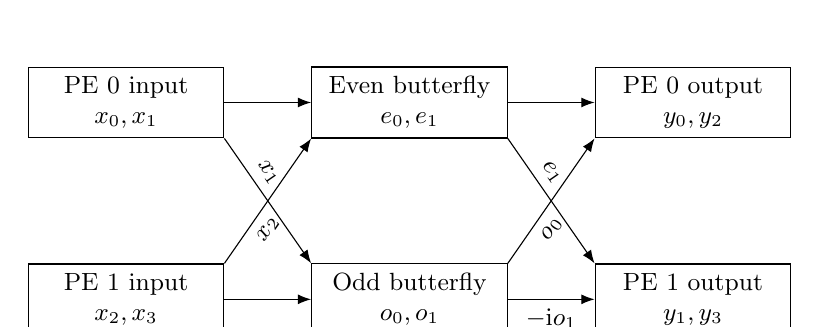
\begin{tikzpicture}[>=Latex,font=\small,box/.style={draw,align=center,minimum height=.85cm,text width=2.25cm}]
\node[box] (a) at (0,1.25) {PE 0 input\\$x_0,x_1$};
\node[box] (b) at (0,-1.25) {PE 1 input\\$x_2,x_3$};
\node[box] (e) at (3.6,1.25) {Even butterfly\\$e_0,e_1$};
\node[box] (o) at (3.6,-1.25) {Odd butterfly\\$o_0,o_1$};
\node[box] (y0) at (7.2,1.25) {PE 0 output\\$y_0,y_2$};
\node[box] (y1) at (7.2,-1.25) {PE 1 output\\$y_1,y_3$};
\draw[->] (a)--(e); \draw[->] (b)--(o);
\draw[->] (e)--(y0); \draw[->] (o)--node[below] {$-\mathrm{i}o_1$} (y1);
\draw[->] (a.south east)--node[pos=.35,above,sloped] {$x_1$} (o.north west);
\draw[->] (b.north east)--node[pos=.35,below,sloped] {$x_2$} (e.south west);
\draw[->] (e.south east)--node[pos=.35,above,sloped] {$e_1$} (y1.north west);
\draw[->] (o.north east)--node[pos=.35,below,sloped] {$o_0$} (y0.south west);
\end{tikzpicture}
\caption{An illustrative two-PE realization of~\eqref{eq:fft}. Horizontal edges stay within a PE; diagonal edges cross ownership. The final frequency layout is interleaved. Routes and buffering are not specified by this diagram.}
\Description{Two rows show two processing elements. Input redistribution and intermediate butterfly values cross between rows before the final butterfly outputs.}
\label{fig:fft}
\end{figure}

\subsection{Hardware reuse is already part of the algebraic tradition}
HSPL explicitly represents streaming and iterative reuse~\cite{milder2012}. In a replication $I_m\otimes A$ for an $n$-input block $A$, width $w$ can realize $w/n$ parallel blocks across $mn/w$ input groups, under the corresponding divisibility assumptions. A cascade can likewise reuse a smaller number of stages through feedback. The paper accounts for streaming permutations and the buffering needed to prevent returning vector data from colliding with an unfinished pass. Its throughput equations assume its pipelined hardware model.

Consequently, neither space/time tradeoffs nor communication-aware transform algebra are missing inventions waiting for a new HLS frontend. Current SPIRAL source also contains distributed gather/send/receive constructs with packet and processor parameters~\cite{spiralsource2026}. A compiler for software-programmed PEs must determine how those structured choices inhabit a different execution contract: instruction issue, local storage, asynchronous operations and their completion conditions. It should retain the algorithmic opportunity while replacing the cost and feasibility model, rather than flattening a formula and later rediscovering its structure.

\subsection{What equivalence permits}
For two exact linear formulas, equality on a basis establishes equality everywhere. The companion checks all 16 coefficients of~\eqref{eq:fft} with Gaussian integers and separately executes its symbolic ownership exchanges. This is a compact illustration of two obligations: formula equality and layout realization. Basis tests do not establish arbitrary-input floating-point equivalence, because rounding does not preserve linearity. Nor do symbolic exchanges prove a physical route can execute. A useful rewrite record therefore includes its algebra, index-map domains, divisibility conditions, numerical policy and input/output layout relations.

The comparison suggests retaining structured formulas, iteration relations and stateful coordination until their useful transformations have been performed. This is a design choice, not a theorem requiring three separate IR implementations. A common IR with sufficiently rich operations, attributes and analyses could preserve the same information. Separate forms make the assumptions easier to inspect; a common representation can reduce conversion overhead and allow optimizations across boundaries. Either approach fails if an early lowering erases the facts needed to justify later transformations.


\section{Compiler Representations and Their Boundaries}\label{sec:compilers}
\subsection{Scheduling a program versus choosing an algorithm}
Halide separates an image algorithm from choices about computation, storage and traversal~\cite{ragankelley2013}. Its two-stage blur illustrates why fusion is not an unconditional improvement: materializing an intermediate exposes parallelism but enlarges reuse distance; full recomputation improves locality at additional work; a sliding window reuses storage while constraining traversal. These alternatives already couple computation with lifetime. Transferring the idea to an array adds a physical ownership question: does an intermediate remain in one memory, or must it cross a PE boundary before its storage can be reclaimed?

Exo externalizes hardware instructions, memories and configuration state into user-level definitions, with schedules expressed as checked rewrites~\cite{exo2022}. Its 2022 core language restricts data-dependent control and models arithmetic over reals; precision and memory checks are separate. Mutable configuration complicates equivalence: a transformation may temporarily preserve behavior only modulo a specified set of global configuration variables. Its analysis tracks this relation, including uncertain loop effects, rather than silently treating configuration writes as pure operations. This is directly relevant to descriptor and execution-state setup in a local PE kernel.

The high-level operation assigned to a custom Exo instruction remains part of the trusted hardware interface. A rewrite checker cannot establish that an incorrectly described instruction implements its declared function. Nor does real-arithmetic equivalence establish bitwise floating-point agreement. Adding a ``send'' intrinsic therefore needs effects, retained-access and completion semantics; a mathematical identity alone cannot justify moving its configuration or reclaiming its operands.

Allo addresses composition through separate compute, memory and communication customization, hierarchical schedules and propagated partition information~\cite{chen2024allo}. Its contribution is complementary to a local scheduling language: a caller and callee must agree on interfaces even when each kernel is individually optimized. Its static equivalence checks apply to the statically interpretable control supported by the method; they do not establish arbitrary runtime progress. For CSL, a useful extension is an interface that states layout, token order and retained storage together. An interface mismatch should either select a compatible specialization or introduce a costed adapter.

\subsection{Data-centric graphs and explicit control}
DaCe's SDFG separates containers, computations and data movement~\cite{bennun2019}. Within a state, memlets specify transferred subsets; maps express parametric parallelism; streams and consume scopes express further execution patterns. State transitions supply sequencing and data-dependent control, and nested SDFGs allow local control inside parallel computation. This directly counters the idea that a graph representation must be a stateless tensor DAG. The original representation also restricts tasklet access to declared connectors, making movement available to transformations instead of hiding it inside arbitrary code.

The resulting boundary is useful: semantic transformations can preserve a tasklet while changing its surrounding memory organization. A new backend still needs a correct interpretation of storage and scheduling annotations. Validation of graph structure and access compatibility is one part of that task. It cannot be cited as a proof of every network-level property introduced by a later CSL or NoC lowering.

Calyx retains hardware structure together with software-like control~\cite{nigam2021}. Components instantiate cells and guarded connections; groups delimit active assignments; \texttt{seq}, \texttt{par}, conditionals and loops determine their activation. The \texttt{go}/\texttt{done} interface gives a completion boundary, while known latency can enable more specialized control. Mutually exclusive groups can share a unit without recovering their schedule from an already flattened state machine. The original IL still requires unique active port drivers; it does not automatically arbitrate every conflicting assignment. A completion-aware PE IR can borrow this separation without claiming that a CSL software task is an RTL group.

\begin{table}[t]
\caption{Representative representations compared by the decision they expose. The final column is the additional question posed by our target problem, not a claim that every listed system lacks all related mechanisms.}
\label{tab:representations}
\small
\begin{tabularx}{\linewidth}{@{}>{\raggedright\arraybackslash}p{2.1cm}XX@{}}
\toprule
Representation & Exposed optimization object & Question at the next boundary \\
\midrule
Alpha / affine IR & Instances, domains and dependence maps & Which finite placement, storage and routes realize the schedule? \\
SPL / Sigma-SPL & Formula alternatives and index composition & Where do indexed values reside after a rewrite? \\
HSPL & Streaming width, iteration and feedback & How do hardware timing assumptions map to local software tasks? \\
Halide / Exo & Storage/computation schedules; checked local rewrites & What protocol connects independently executing regions? \\
SDFG / Allo & Data movement, state or compositional customization & Which interface facts must a target adapter preserve? \\
Calyx / elastic HLS & Activation, completion, handshakes and resource use & What is the actual backend's ownership and progress contract? \\
AIR / TL & Async hierarchy or tile-to-core mapping & Which resource limits and cost estimates are target-specific? \\
\bottomrule
\end{tabularx}
\end{table}

\subsection{Static regions inside dynamic execution}
Dynamatic lowers C/C++ to circuits whose operators synchronize through handshakes~\cite{josipovic2020}. Dynamic scheduling can exploit runtime readiness, but channels, steering logic and buffers consume resources. A statically scheduled region can avoid some of this overhead when its timing and dependencies are predictable. DASS explicitly investigates this mixed approach~\cite{cheng2021dass}. The important unit of comparison is therefore the region and its interface, rather than a forced choice between an entirely static or entirely dynamic application.

Sharing also changes the execution graph. CRUSH assumes a deadlock-free circuit before sharing and prevents deadlocks introduced by its sharing mechanism~\cite{crush2025}. It reserves per-operation output capacity with credits and returns credits when results leave the corresponding output buffer. Ready requests can proceed when a higher-priority request is absent; a fixed required access order could otherwise create a new wait cycle. Sufficient buffering for throughput is a further question after correctness. This is a precise precedent for separating credit safety from performance, with a narrower theorem than unconditional deadlock freedom for arbitrary circuits.

For software PEs, the analogous resource may be a vector unit, task slot or communication engine. Moving two independent actors onto one PE introduces serialization and potentially a new wait relation. The compiler should recheck the composed resource protocol, even if both actors passed local checks before folding. Conversely, two operations sharing one arithmetic unit need not share all their state, completion identities or output queues.

\subsection{Infrastructure is not a semantic proof}
MLIR permits domain-specific operations, types and staged lowering within common compiler infrastructure~\cite{lattner2021}. Its Transform dialect provides a programmatic way to apply transformations to payload IR~\cite{mlirtransform2026}. Neither the presence of SSA values nor a transform script gives a graph its firing semantics. Operation verification, transformation legality and backend operational correctness must each be defined. Experience from building Dynamatic on MLIR illustrates that an infrastructure designed for software does not remove the representational demands of HLS~\cite{xu2026mlir}.

AIR exposes hierarchy and asynchronous dependencies through launch, segment, herd, channel and token constructs~\cite{wang2025air}. TL instead studies how tile instances, affine accesses and reuse map onto a spatial grid, with capacity pruning, cost-based ranking and optional profiling~\cite{li2025tl}. These are complementary contributions: an asynchronous plan can provide executable coordination, while a mapping search can choose placement and reuse. Their composition requires a cost model whose overlaps are legal under that coordination. Predicted transfer/compute overlap is invalid when the actual program serializes the operations or holds the buffer that the next transfer needs.

No universal winner follows from Table~\ref{tab:representations}. Higher-level forms expose powerful domain rewrites but restrict expressiveness. Lower-level forms make implementation choices explicit but can make equivalence harder to recover. A practical compiler should define where each transformation is justified, what facts survive lowering, and what information a failed later analysis returns to an earlier search stage.


\section{A Worked Dependence-to-Protocol Chain}\label{sec:gemm}
\subsection{The mathematical program}
Let $A\in\R^{M\times K}$ and $B\in\R^{K\times N}$. Define the iteration domain
\begin{equation}
 D=\{(i,j,k)\in\Z^3:0\le i<M,\ 0\le j<N,\ 0\le k<K\}.
\end{equation}
A recurrence exposes the reduction order:
\begin{equation}\label{eq:gemm}
 c_{ij}^{(0)}=0,\qquad c_{ij}^{(k+1)}=c_{ij}^{(k)}+A_{ik}B_{kj}.
\end{equation}
Induction on $k$ gives $c_{ij}^{(K)}=(AB)_{ij}$ in exact arithmetic. Dependences connect consecutive accumulator versions. Operand reuse can be implemented as repeated memory reads, multicast, or explicit forwarding; those alternatives have the same mathematical input but different communication graphs. Adding forwarding edges is a realization decision, not a property forced by the original equation.

\subsection{Unfolded systolic placement}
For one realization, place $(i,j,k)$ at $\pi(i,j,k)=(i,j)$ and schedule its MAC issue at
\begin{equation}\label{eq:theta}
 \theta(i,j,k)=i+j+Lk.
\end{equation}
Here $L\ge1$ is the assumed recurrence latency in logical time units. Assume independent operand forwarding, one unit per neighbor hop, and sufficient issue and link resources. Inject $A_{ik}$ at the west boundary at $i+Lk$ and $B_{kj}$ at the north boundary at $j+Lk$. Each arrives at PE $(i,j)$ at $\theta(i,j,k)$. Accumulator dependences have distance $L$; horizontal and vertical forwarding dependences have distance one. These equations establish feasibility only for this explicitly idealized profile. They do not estimate CSL instruction cycles or a measured interconnect latency.

A folded map needs a new resource argument. Mapping all operations of a $2\times2$ grid to one single-issue PE while retaining~\eqref{eq:theta} assigns $(0,1,0)$ and $(1,0,0)$ to the same resource at time one. No algebraic or dependence-order error is required for this conflict. An additional serialization schedule, feasible routes and sufficient buffering must be found.

\subsection{Blocked SUMMA on the existing backend}
The implemented Pragma profile instead uses a $P\times P$ grid with $M=Pm_t$, $K=Pk_t$ and $N=Pn_t$. PE $(x,y)$ owns an $m_t\times n_t$ output block. At round $r$, it obtains an $A$ panel from column $r$ of its row and a $B$ panel from row $r$ of its column, then accumulates the $k_t$ corresponding products. If $C_{xy}^{[r]}$ is the resident block after $r$ rounds,
\begin{equation}\label{eq:summa}
 C_{xy}^{[0]}=0,\qquad
 C_{xy}^{[r+1]}=C_{xy}^{[r]}+A_{yr}B_{rx}.
\end{equation}
By induction, the block contains the partial product through global reduction index $rk_t-1$. This induction concerns values. It also requires the implementation to supply the correct panel versions and to preserve their storage during computation.


\subsection{From panels to an execution contract}
The panel-value induction requires the correct versions of both inputs to be ready, and their storage to remain unchanged throughout the local computation. The companion models separate transfer completions, reader borrows and the release that permits the next round. Appendix~\ref{app:protocol} gives the finite operational model and its conditional proof. Section~\ref{sec:backends} relates the event order to concrete target interfaces; no automatic semantics extraction from CSL is claimed.

\subsection{Acyclic dataflow can deadlock with bounded writes}\label{sec:deadlock}
Consider two initially empty FIFO edges $a,b$ from producer $P$ to consumer $Q$. The programs are

\begin{lstlisting}[float=htbp,caption={A balanced but incompatible stream order.}]
P: put(a); put(a); put(b)
Q: get(b); get(a); get(a)
\end{lstlisting}

Both actors agree on the numbers of tokens. With capacity one on each edge, $P$ can perform its first write, but its second write blocks; $Q$ blocks on $b$. The data graph is acyclic, yet backpressure creates a wait cycle. Capacity two on $a$ repairs this program. Changing the producer's order to $a,b,a$ is a distinct repair. Rate balance and graph acyclicity do not choose between them.

Here FIFO operations publish and reclaim atomically. They are not a model of an asynchronous DMA with a retained input borrow. The timed CSDF model discussed in Section~\ref{sec:rates} already distinguishes output reservation from input-credit return~\cite{stuijk2008}. Its firing-time assumptions must be checked when relating it to a particular asynchronous implementation.

\subsection{Numerical equivalence is a separate obligation}
The exact-arithmetic recurrence does not license arbitrary floating-point reassociation. With binary32 rounding, $a=2^{24}$, $b=1$ and $c=-2^{24}$ give $(a+b)+c=0$ but $a+(b+c)=1$. The prototype reproduces this counterexample using explicit binary32 rounding. The existing backend therefore retains its explicit relaxed-FMA policy and componentwise error check. An ownership proof cannot establish a numerical tolerance.



\section{Three Concrete Execution Contracts}\label{sec:backends}
An asynchronous edge needs several meanings: reserving destination storage, initiating transfer, making the value visible, ending an access and permitting reuse. Different targets combine these events differently. Table~\ref{tab:backends} compares inspected interfaces; it is not a claim that one universal FIFO API can replace them.

\begin{table}[t]
\caption{Backend-specific facts that must survive lowering. Software observations are pinned or dated in Appendix~\ref{app:sources}; no AIE or Metalium experiment was performed for this survey.}
\label{tab:backends}
\small
\begin{tabularx}{\linewidth}{@{}>{\raggedright\arraybackslash}p{1.6cm}XXX@{}}
\toprule
Backend & Local execution & Communication boundary & Reuse obligation \\
\midrule
CSL, WSE-3 & Tasks, vector operations, DSD/DSR resources & Fabric queues, routes, async completion and collective interfaces & Preserve buffers and descriptors until their relevant users finish \\
AIE / IRON & Worker code and object acquisition & ObjectFifo endpoints lowered into buffers, locks and DMA resources & Release acquired objects only after the local use is complete \\
Metalium & Data-movement and compute kernels & Circular buffers and NoC operations/barriers & Publish after incoming data arrives; reclaim after retained data is no longer accessed \\
\bottomrule
\end{tabularx}
\end{table}

\subsection{Cerebras CSL: readiness and vector state}
CSL exposes PE-local code together with fabric configuration. On the inspected WSE-3 interface, data tasks are associated with input queues; local tasks have explicit identities. A task's activation and blocking state are distinct: activation alone does not make a blocked task execute~\cite{csltasks2026}. This distinction can implement a join, but the compiler must initialize and restore the states correctly across repeated invocations. It must not substitute an assumed counting semaphore for the documented task interface.

Data structure descriptors (DSDs) describe memory or fabric operands; loading them into data structure registers (DSRs) associates operations with finite execution state~\cite{csldsd2026}. An asynchronous vector operation can signal completion by activation or unblocking. Descriptor banks, fabric queues and microthreads are resources, not merely annotations on a mathematical vector operation. A proposed overlap needs compatible allocations and must preserve the relevant descriptor and operand state until completion. The current public documentation contains a queue-sharing discrepancy between its DSD and microthread descriptions; Appendix~\ref{app:sources} records it. The companion conservatively uses distinct resources for the two panel transfers.

The existing SUMMA template uses separate completion paths: one activates an initially blocked compute task and the other unblocks it. The compute task restores the block before the next round. A reviewed abstraction can model this as waiting for two distinct events, provided the event-to-task relation and the SDK collective guarantees are stated. It is not legitimate to infer that any local send completion means the remote computation has finished using the value.


\begin{lstlisting}[float=htbp,caption={Actual completion handlers in the companion CSL template; initialization and the compute body are omitted.}]
task x_done() void { @activate(compute_task_id); }
task y_done() void { @unblock(compute_task_id); }
// Initially, and before the next round:
// @block(compute_task_id);
\end{lstlisting}


CSL's current SdkLayout API already offers rectangular CodeRegions, ports and automatic route/color assignment~\cite{cslregions2026}. A higher-level compiler should use and validate these facilities where appropriate. Its additional responsibility is to derive region contents, compatible interfaces and global execution obligations from an algorithm. Reimplementing region composition under a new name would not establish that contribution.

\subsection{AMD AI Engines: object ownership through lowering}
IRON exposes workers and ObjectFifo handles over the MLIR-AIE infrastructure~\cite{iron2025}. Acquiring an object grants access to storage whose availability is synchronized; releasing it advances the ownership protocol. In the inspected handle API, an acquire count is the number of objects requested to be held, not an unconditional increment on every call~\cite{aiesource2026}. Thus, with one object already held, requesting two acquires the additional availability required for two, subject to the interface rules. Treating this as two destructive pops changes the protocol.

The pinned development pipeline splits and verifies object FIFOs, allocates resources, lowers DMA and core operations, then removes the higher-level objects. Core lowering tracks acquired objects and emits lock operations; its concrete implementation depends on architecture and repeat settings. The simple interpretation here concerns repeat factor one. A compiler using this layer can preserve an abstract acquire/use/release contract while delegating lock and DMA construction. It must still ensure that worker access patterns and object counts satisfy that contract. Structural verification is not a proof of progress for every combination of workers and external streams.


\begin{lstlisting}[float=htbp,caption={A worker-side use of the pinned ObjectFifoHandle API. The named handles and synchronous kernel are supplied by the enclosing program.}]
a = a_cons.acquire(1)
b = b_cons.acquire(1)
local_kernel(a, b)
a_cons.release(1)
b_cons.release(1)
\end{lstlisting}

Both channels start with no acquired objects, and the kernel retains neither pointer after returning. If it launches asynchronous work, return from the call alone is insufficient to justify either release. The generated locks manage object availability; the worker body remains responsible for the declared use interval.

\subsection{Tenstorrent: publication and NoC completion}
Metalium makes circular-buffer ownership and NoC completion explicit~\cite{ttsource2026}. A producer reserves space before filling it and publishes completed entries afterward. A consumer waits for available entries, accesses them, and pops them when reclamation is safe. NoC barriers concern specified transfer completion; publication and application-level consumption remain separate events. These selected statements are from the pinned reader; the intervening reads are described below:

\begin{lstlisting}[float=htbp,caption={Reservation and publication statements from the Metalium reader, with the intervening transfer calls omitted.}]
cb_in0_buf.reserve_back(1);
cb_in1_buf.reserve_back(1);
// Two noc.async_read(...) calls occur here.
noc.async_read_barrier();
cb_in0_buf.push_back(1);
cb_in1_buf.push_back(1);
\end{lstlisting}

The pinned reader example uses the newer Noc/CircularBuffer wrappers to reserve two inputs, issue both reads, wait for the reads and publish both inputs. The low-level API exposes the corresponding \texttt{cb\_reserve\_back}, \texttt{cb\_push\_back}, \texttt{cb\_wait\_front} and \texttt{cb\_pop\_front} operations. A NoC write-completion guarantee should not be relabeled as the destination algorithm's acknowledgement. This distinction determines when a producer may recycle a source slot and when a receiver may recycle its destination slot.

\subsection{A common contract without a false common machine}
Our synthesis is to model a communicated value as a versioned object with a producer reservation, publication event, reader borrows and reclamation condition. A backend may collapse events when its documented semantics permits it. For an atomic FIFO, publication and a write can coincide; for a DMA they need not. A shared immutable object may have several readers; a destructive stream read has different ownership. A target adapter should state the abstraction relation rather than relying on operation names such as ``wait'' or ``done.''

For example, the following logical contract can have several implementations:
\begin{equation}\label{eq:borrow}
 \operatorname{reserve}(b,v)\hb\operatorname{publish}(b,v)
 \hb\operatorname{borrow}_j(b,v)\hb\operatorname{release}_j(b,v).
\end{equation}
Reusing $b$ for $v+1$ requires every relevant release for $v$, as well as completion of retained hardware accesses. This partial order is a safety specification. It does not allocate a route, establish fairness, or bound waiting time. Those obligations remain visible in the physical plan instead of being silently discharged by a common graph syntax.

Consider a common two-input trace: $A_v$ becomes ready, $B_v$ becomes ready, a local kernel reads both, then the two input slots become reusable. CSL realizes the join with the two task-state changes above; the collective completion contract supplies readiness. IRON realizes it by obtaining both consumer handles before the synchronous call and releasing them afterward. In Metalium, the reader's barrier precedes publication, and the compute consumer separately waits for both buffers and pops after its final use. None of these implementations requires the two transfers to complete in the same order. None permits a producer to infer consumption from publication. The shared partial order is therefore portable; the task, lock and NoC mechanisms implementing it are not interchangeable instructions.


\section{Workloads That Test the Abstraction}\label{sec:applications}
Algorithm families exercise different constructive choices. Dense products expose reuse and reduction; interval dynamic programming couples a regular domain to a growing dependence frontier; sparse products make access coordinates input-dependent; numerical solvers add reusable factors, convergence and persistent vectors; attention changes the reduction state to avoid a large intermediate. The comparison below asks both how a useful spatial organization is obtained and what information its implementation requires.

\subsection{Interval dynamic programming has a regular but expanding frontier}
For a finite interval problem, consider
\begin{equation}\label{eq:interval-dp}
 c(i,j)=\min_{i<k<j}\{c(i,k)+c(k,j)+w(i,k,j)\},
 \qquad c(i,i+1)=c_i^0.
\end{equation}
The branch selected by the minimum depends on values, but the candidate index set is statically known. With $d=j-i$, every candidate reads shorter intervals. A length-ordered traversal therefore exposes a legal wavefront. A direct realization stores completed diagonals and scans the candidates; a more spatial realization distributes candidate comparisons and pipelines completed interval values toward their future consumers. The variable reduction length and the two operand frontiers are the design problem, not the scalar minimum instruction.

Dhrif and Sarkar study this recurrence family through matrix-chain ordering~\cite{dhrif1992}. Their linear-array organization completes one diagonal stage at a time; the stages have unequal durations and require varying local storage. Their mesh organization overlaps diagonals and forwards completed entries, trading more processors for constant local computation state. The paper reports $O(n^2)$ time with $O(n)$ processors and $O(n)$ time with $O(n^2)$ processors in its respective models. The latter includes six-neighbor geometric connectivity and unit-step communication/computation assumptions. Those bounds are not measured four-neighbor wafer results. Its matrix-chain input can be generated from a short dimension vector; an arbitrary independently supplied $w(i,k,j)$ table has a different input-volume problem.

Our synthesis consequence is to keep the reduction frontier and the operand-generation rule explicit. The abstract recurrence alone does not price weight delivery or embed a six-neighbor graph into a physical mesh. If the output includes the optimal parenthesization, each minimum must also preserve an argmin and a tie rule; retaining or recomputing that reconstruction information is an additional choice. This workload separates value-dependent selection within a regular index domain from the data-dependent coordinate traversal of sparse formats.

\subsection{Sparse iteration is not a dense loop with zeros removed}
For a compressed sparse row (CSR) matrix with unique column coordinates within each row, the mathematical product is
\begin{equation}\label{eq:csr}
 y_i=\sum_{p=\mathrm{rowptr}[i]}^{\mathrm{rowptr}[i+1]-1}
       \mathrm{val}[p]x_{\mathrm{col}[p]}.
\end{equation}
The loop over stored positions and the access to logical coordinates are different maps. In particular, $\mathrm{col}[p]$ is input data, not generally an affine expression in $p$. A source contract must specify index bounds, duplicate handling and whether implicit entries denote algebraic zeros. The latter matters for machine arithmetic: omitting $0\cdot\mathrm{NaN}$ is not equivalent to executing that IEEE operation.

TACO's 2017 representation combines tensor index expressions with storage-level iteration~\cite{taco2017}. Iteration graphs encode the access order imposed by each operand's format. Merge lattices organize simultaneous iteration: addition typically requires a union of stored coordinates, multiplication an intersection under the zero-annihilator assumption. An expression such as $(b_i+c_i)d_i$ requires combinations of these cases. Its original code generator requires an acyclic iteration graph; conflicting format orders can require conversion. These mechanisms provide information that a generic tensor DAG or affine-only loop representation does not supply.

The following is our illustrative row-owned PE program, not generated TACO or CSL code:

\begin{lstlisting}[float=htbp,caption={Sparse matrix--vector multiplication with an explicit remote-value contract.}]
for i in owned_rows:
    acc = 0
    for p in range(rowptr[i], rowptr[i + 1]):
        value = obtain_x(col[p], iteration_version)
        acc += val[p] * value
    publish_y(i, acc, iteration_version)
\end{lstlisting}

The unresolved operation is \texttt{obtain\_x}. Replicating the full vector replaces communication with resident storage. A structure-specific inspector can precompute required remote coordinates and exchange lists when the sparsity pattern persists. A dynamic request/reply implementation instead needs bounded outstanding requests, reply storage and a progress argument. These are alternative designs, not interchangeable lowerings of an unqualified array read. Splitting a long row among PEs additionally changes the reduction order and requires an output-combination protocol. A useful compiler interface therefore preserves both coordinate semantics and the choice of ownership strategy.

\subsection{Factorization changes the reduction object}
Gentleman and Kung's triangularization arrays expose an instructive alternative to a dense block pipeline~\cite{gentleman1982}. Boundary cells determine a transformation that eliminates an incoming element; interior cells apply it to the remaining row entries. The same geometric framework supports different elimination operations. In the Givens case, square roots and reciprocals make boundary cells more expensive than multiply/add interior cells. The paper discusses square-root-free variants that change scaling operations and diagonal communication. Thus arithmetic formulation and array throughput are coupled design decisions.

Using our real-arithmetic sign convention, an incoming row $x$ updates a stored triangular factor $R$ column by column. At boundary $k$, let $\rho=\sqrt{r_{kk}^2+x_k^2}$. For $\rho>0$, choose $c=r_{kk}/\rho$, $s=x_k/\rho$, so
\begin{equation}\label{eq:givens}
 G=\begin{bmatrix}c&s\\-s&c\end{bmatrix},\qquad
 G\begin{bmatrix}r_{kk}\\x_k\end{bmatrix}
 =\begin{bmatrix}\rho\\0\end{bmatrix},\qquad G^TG=I.
\end{equation}
For $\rho=0$, use the identity transformation. Each interior cell $j>k$ applies the same $G$ to $(r_{kj},x_j)$, retaining the first result and forwarding the second toward later elimination. In machine arithmetic, a scaled hypotenuse computation and a numerical policy are needed; naively squaring large entries can overflow.


\begin{lstlisting}[float=htbp,caption={Derived real-arithmetic state update for one row; the simultaneous use of old values is essential.}]
for k in range(num_columns):
    rho, c, s = givens_parameters(R[k,k], x[k])
    R[k,k], x[k] = rho, 0
    for j in range(k+1, num_columns):
        r_old, x_old = R[k,j], x[j]
        R[k,j] = c*r_old + s*x_old
        x[j]   = -s*r_old + c*x_old
\end{lstlisting}

The spatial realization sends rotation parameters along the row and routes updated entries to subsequent boundary cells. Its persistent state is the triangular factor; processing an additional row updates that state. An appended right-hand-side column can undergo the same transformations for least squares. Whether the application needs only the updated $R$, a transformed right-hand side or a reusable representation of $Q$ changes what must be retained. A heterogeneous PE assignment can reserve more resources for boundary work; changing the rotation algorithm is a different response to the same bottleneck.

For tall matrices already available as blocks, TSQR offers another organization. It factors block rows locally, then factors stacks of their triangular factors along a tree~\cite{demmel2008}. For two blocks, thin local factorizations give
\begin{equation}
 \begin{bmatrix}A_0\\A_1\end{bmatrix}
 =\begin{bmatrix}Q_0&0\\0&Q_1\end{bmatrix}
  \begin{bmatrix}R_0\\R_1\end{bmatrix}
 =\begin{bmatrix}Q_0&0\\0&Q_1\end{bmatrix}\widehat Q R.
\end{equation}
The reduction communicates triangular factors rather than complete block rows. If the application later applies $Q$ or $Q^T$, the intermediate orthogonal transformations and their tree association must remain available. The TSQR report explicitly discusses this requirement, which a result-only reduction interface would hide. Thus output liveness depends on the downstream operation: ``compute $R$'' and ``produce a reusable QR factorization'' have different storage contracts.

Our compiler implication is to retain an algorithm-level factorization object until its future uses are known. Replacing Householder QR with a Gram-matrix-based method merely because matrix multiplication is efficient changes the numerical problem: in exact arithmetic, for full-column-rank $A$, $\kappa_2(A^TA)=\kappa_2(A)^2$. The availability of a fast product does not justify that substitution. Similarly, an LU interface must state its pivoting policy and permutation output; a no-pivot implementation is a specialization with additional input assumptions. These choices belong above instruction selection and network scheduling.

\subsection{Iterative solvers require distributed decisions}
For an SPD system, a conventional unpreconditioned CG iteration includes
\begin{align}
 q_k&=Ap_k,& \alpha_k&=(r_k^Tr_k)/(p_k^Tq_k),\\
 x_{k+1}&=x_k+\alpha_kp_k,&r_{k+1}&=r_k-\alpha_kq_k,\\
 \beta_k&=(r_{k+1}^Tr_{k+1})/(r_k^Tr_k),&
 p_{k+1}&=r_{k+1}+\beta_kp_k.
\end{align}
These equations assume the iteration has not already converged and the denominators are valid. The Templates treatment identifies inner products as synchronization points and distinguishes the communication properties of preconditioners~\cite{templates1994}. The algorithm is therefore not established by separately testing SpMV, dot and vector updates.

For a spatial implementation, the scalar reduction must reach every PE that updates the associated vector version. A convergence decision must select the same branch across participants before channels or buffers are reset. Speculatively starting an iteration requires either guaranteeing its consumption or defining cancellation that drains or invalidates its in-flight data. A preconditioner is itself a program: diagonal scaling and a distributed triangular solve impose different dependence graphs. Pipelined or communication-avoiding solver variants should enter as algorithm alternatives with their own numerical analysis, not as an unexamined overlap optimization. This is also why a fixed iteration-count demonstration is weaker than a solver with tested stopping, breakdown and restart behavior.

\subsection{Attention as a stateful reduction}
FlashAttention demonstrates that exact attention can be reorganized around blocks and normalization statistics without materializing the full score matrix~\cite{flash2022}. The underlying combination can be written explicitly. For one query and a nonempty set $J$ of finite scores $s_j=q^Tk_j/\sqrt d$, define
\begin{equation}
 m_J=\max_{j\in J}s_j,\quad
 \ell_J=\sum_{j\in J}e^{s_j-m_J},\quad
 z_J=\sum_{j\in J}e^{s_j-m_J}v_j.
\end{equation}
For disjoint nonempty blocks $U,V$, let $m=\max(m_U,m_V)$. Then
\begin{equation}\label{eq:softmax-merge}
 (m_U,\ell_U,z_U)\oplus(m_V,\ell_V,z_V)
 =\left(m,\ e^{m_U-m}\ell_U+e^{m_V-m}\ell_V,
             e^{m_U-m}z_U+e^{m_V-m}z_V\right).
\end{equation}
Rescaling each summand establishes that this is the state for $U\cup V$; the output is $z/\ell$. In real arithmetic, combination is associative on these valid states. Empty or fully masked blocks need an explicit identity case, avoiding the undefined subtraction $-\infty-(-\infty)$. Floating-point merge trees need a separate accuracy analysis.

The spatial choice is now concrete: stream blocks through one accumulator, distribute partial states and reduce them, or replicate queries while partitioning keys. Each has a different state size, communication volume and critical path. An implementation must keep the three statistics mutually consistent; publishing an updated maximum with an old numerator exposes an invalid state. Kernel fusion can preserve this atomicity locally, while a multi-PE realization needs a versioned aggregate interface. The algebra permits alternatives but does not select a route or establish a numerical tolerance.

\subsection{Wafer-scale execution adds persistent layout and code}
WaferLLM makes parallelism, nonuniform access latency, local memory and routing resources explicit in its PLMR model~\cite{he2025}. Its MeshGEMM combines cyclic movement with an interleaved physical placement; MeshGEMV uses hierarchical reduction. Prefill and decode use different layouts and PE allocations. Its KV-cache shift distributes growing state across neighboring rows instead of concentrating appended entries. The reported complete-model experiments include LLaMA3-8B and LLaMA2-13B on WSE-2; the larger 34B/72B cases use subsets of layers for the corresponding operator/phase measurements. These are paper results, not experiments reproduced here, and do not establish multi-request serving behavior.

Our implication is that a model-level compiler must optimize transitions between operators and phases as well as each operator. For $L$ layers with a common number $H_{kv}$ of KV heads, head dimension $d$, element size $b$ bytes, and active request lengths $S_u$, uncompressed KV payload alone requires
\begin{equation}\label{eq:kv}
 M_{KV}=2LH_{kv}db\sum_u S_u.
\end{equation}
This excludes weights, allocator overhead, temporary activations and replication. A feasible total does not imply a feasible placement: every PE must fit its assigned peak live state. Request identity and layer/token versions prevent cross-request aliasing; admission, eviction and reset are additional runtime policies. Weight residency and KV residency should be independent decisions in the interface. Nothing in a single-request operator demonstration determines a commercial deployment's policy.

MACH exposes another resource often absent from tensor-level cost models: the control program itself~\cite{vanessendelft2025}. Its controller/worker organization broadcasts operation selections and arguments while workers retain reusable operation definitions. The paper lowers through Tungsten and Paint; this is not evidence of a public CSL backend. Nonparticipating workers still consume their broadcast arguments to avoid blocking the stream. This illustrates that an actor with no numerical contribution can have an essential protocol role.

For our proposed HLS, reusable local kernels and a compact control representation are alternatives to repeatedly expanding a large graph. The cost model must include instruction storage, descriptors, control traffic and argument consumption alongside tensor buffers. A phase boundary is safe only when its retained hardware accesses and required stream consumption have completed. The workload analysis therefore returns to the same distinction: values define the requested computation; ownership, control and progress define its executable realization.


\section{Compiler Design Synthesis}\label{sec:design}
\subsection{A search space derived from the algorithm families}
The survey supports a compiler organized around a hierarchy of alternatives, rather than an operator catalogue followed by one mapping pass. Table~\ref{tab:constructive-comparison} summarizes the constructive choices exposed by the worked families. The rows are not interchangeable optimization recipes: each has a different equivalence relation and a different state object.

\begin{table}[ht]
\caption{Constructive choices and the information needed to compare them. These are synthesis conclusions from the preceding derivations, not implemented Pragma features.}
\label{tab:constructive-comparison}
\small
\begin{tabularx}{\linewidth}{@{}>{\raggedright\arraybackslash}p{1.55cm}XX@{}}
\toprule
Family & Algorithm or spatial alternative & Decision-relevant information \\
\midrule
FIR & Propagation chain; folded tap scan & Reuse direction, input rate, sample history, stream alignment \\
FFT & Factorization; permutation absorption; temporal reuse & Factor dimensions, index maps, arithmetic policy, exchange volume \\
GEMM & Neighbor forwarding; blocked panel collectives & Operand replication, tile lifetime, recurrence latency, link contention \\
LU/QR & Invariant choice; streaming rotations; block/tree reduction & Pivot or rotation policy, retained factors, boundary cost, downstream uses \\
Interval DP & Stored frontier; overlapping diagonal pipelines & Candidate domains, weight generation, topology, reconstruction state \\
Sparse & Replication; inspected exchanges; dynamic requests & Coordinate structure, skew, remote ownership, outstanding-use limits \\
CG & Conventional recurrence; preconditioned or communication-reduced variant & Convergence, numerical stability, reduction dependencies, iteration state \\
Attention & Streaming statistic; distributed merge; query replication & Stable normalization state, KV placement, phase transitions, request lifetimes \\
\bottomrule
\end{tabularx}
\end{table}

At the highest level, a domain library should express families of valid decompositions: FLAME-style invariant choices, SPIRAL-style factorizations or an application-specific stable reduction. At the next level, localization and traversal construct communication opportunities. Projection, tiling, folding and retiming then select how much computation and delayed state are spatial or temporal. A target-aware layer resolves resource conflicts and operational interfaces. Feedback may cross several levels: a QR boundary bottleneck can motivate a different rotation implementation or algorithm; a long propagation route can motivate a new localization basis; an oversized live frontier can motivate a different factorization or traversal.

This separation makes a concrete research distinction. Reusing a verified rewrite rule is different from reusing a placement heuristic, and neither automatically supplies a numerical acceptance criterion. A useful implementation should expose enough structured alternatives to compare these choices without requiring users to rewrite every PE program. The literature already contains the ingredients; the project-specific challenge is integrating selected methods and making their interactions experimentally accountable.

\subsection{Proof boundaries should follow semantic boundaries}
ATL verifies high-level tensor rewrites using a Coq embedding with real-number semantics~\cite{atl2022}. Its shape reasoning and reshaping operations make a useful distinction between the value-level transformation and eventual storage layout. The 2022 paper identifies verification of lower-level compilation as further work. It should consequently be cited for the transformations it verifies, not as proof of an entire floating-point spatial implementation. Exo's checked local rewrites and Allo's static equivalence checking likewise address specified subproblems, with different source-language assumptions.

ElasticMiter addresses a different boundary: equivalence of latency-insensitive circuits~\cite{elasticmiter2025}. Its comparison includes input consumption as well as output values, allowing the two circuits to consume and produce at different times. Decoupling and nondeterministic delays expose mismatches that cycle-aligned output comparison misses. Eventual propagation and the modeled context matter to the progress property. This is a useful precedent for validating a schedule-changing refinement. It is substantially stronger than selecting a few successful input schedules, and is not what the companion's finite protocol checker implements.

These results suggest composing obligations explicitly. A value rewrite establishes a relation between algorithms. A schedule establishes dependence legality under the selected numerical policy. A storage rewrite establishes a relation between logical versions and physical addresses. A communication lowering preserves publication and use order under backend assumptions. Finally, progress excludes permanent valid-prefix execution. Passing one layer should not silently remove the next layer's obligation.

\subsection{A proposed constructive compilation pipeline}
Figure~\ref{fig:design} organizes our proposed compiler. It is a research design derived from the comparisons, not a description of a fully implemented Pragma pipeline. The stages can be separate IRs or different views within one extensible IR. The requirement is that the relevant facts remain available and transformations have explicit preconditions.

\begin{figure}[t]
\centering
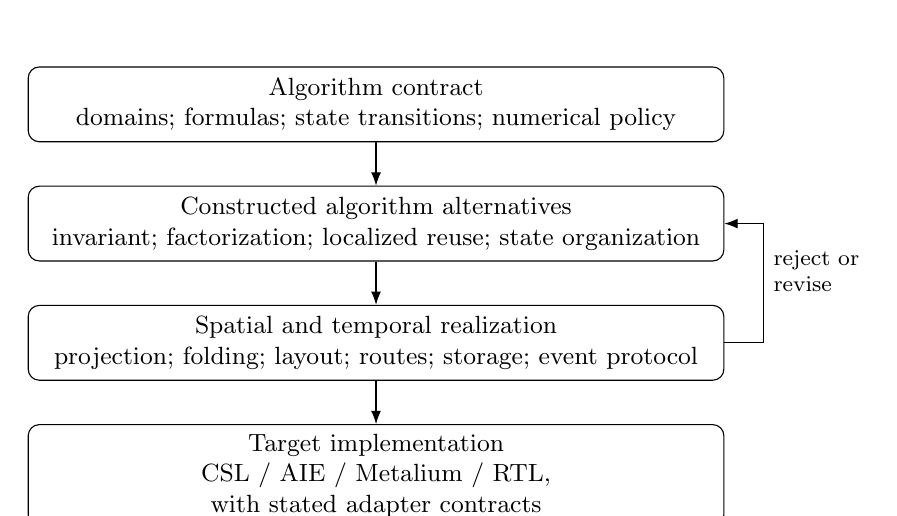
\begin{tikzpicture}[font=\small,>=Latex,
 stage/.style={draw,rounded corners,align=center,text width=8.6cm,minimum height=.95cm}]
\node[stage] (a) {Algorithm contract\\domains; formulas; state transitions; numerical policy};
\node[stage,below=.55cm of a] (b) {Constructed algorithm alternatives\\invariant; factorization; localized reuse; state organization};
\node[stage,below=.55cm of b] (c) {Spatial and temporal realization\\projection; folding; layout; routes; storage; event protocol};
\node[stage,below=.55cm of c] (d) {Target implementation\\CSL / AIE / Metalium / RTL, with stated adapter contracts};
\draw[->] (a) -- (b);
\draw[->] (b) -- (c);
\draw[->] (c) -- (d);
\draw[->] (c.east) -- ++(.5,0) |- node[pos=.3,right,align=left,font=\footnotesize]{reject or\\revise} (b.east);
\end{tikzpicture}
\caption{Proposed compilation with feedback from physical feasibility to algorithm and schedule selection. Numerical, safety and progress obligations accompany the transformations; the boxes are not implemented-feature claims.}
\Description{Four stages run from the algorithm contract through alternatives and a physical plan to a target implementation. An arrow returns a failed physical plan to the alternatives stage.}
\label{fig:design}
\end{figure}

At the algorithm boundary, an operation declares domains and effects, including persistent state. A transform can select a factorization, change a traversal or introduce temporary storage only under its declared equivalence relation. For example, a permutation may be absorbed into a consumer's layout if the interface changes consistently; otherwise it requires an explicit adapter. A reduction-tree rewrite may be valid over reals but unavailable under strict floating-point ordering. Sparse format conversion changes physical representation while preserving coordinate meaning, subject to duplicate and implicit-zero semantics.

At the region boundary, a producer and consumer agree on logical indices, value versions, physical layouts and use intervals. We propose a contract of the form
\begin{equation}
 \mathcal C=(D,\tau,\nu,\lambda,\rho,E,\Omega),
\end{equation}
where $D$ is the coordinate domain, $\tau$ the element type, $\nu$ the numerical relation, $\lambda$ the ownership/layout map, $\rho$ the production/consumption pattern, $E$ the visible effects, and $\Omega$ the completion and reclamation conditions. This is a specification schema, not a claim that seven fields suffice for every dynamic program. Parameters or predicates must represent conditional behavior; an unknown rate must not be replaced with a fabricated fixed rate.

At the execution boundary, the plan identifies concrete resources and a backend adapter identifies the operational meaning of each action. A plan using a synchronous local kernel can release a borrow at return. An asynchronous kernel must return an outstanding-use event or retain the borrow until a later completion. Aliased views of one allocation must share the same underlying ownership accounting. A wrapper that labels an unsafe operation ``async copy'' has not discharged these conditions.

\subsection{Search guidance and final acceptance are different}
Let a candidate $c$ contain an algorithm alternative, a numerical policy and a physical plan. Legality is a conjunction of predicates rather than a single weighted cost:
\begin{equation}
 \mathcal F(c)=\mathcal V(c)\land\mathcal N(c)\land\mathcal D(c)
 \land\mathcal M(c)\land\mathcal R(c)\land\mathcal P(c),
\end{equation}
representing value/effect semantics, numerical admissibility, dependence order, memory, resource feasibility, and protocol safety/progress under stated assumptions. Some predicates may be unknown. A timed-out solver or exhausted model checker therefore yields an unresolved candidate, not evidence of legality or impossibility. These are final-acceptance conditions, not a required search order. Cost-guided search may rank partial or temporarily infeasible candidates, as DRESC's penalized resource overuse illustrates. The distinction is between an exploratory candidate and a released implementation that relies on a property already being established.

Memory feasibility is local and temporal. For PE $p$, physical live allocations $\mathcal L_p(t)$ with sizes $s_a$ must satisfy
\begin{equation}\label{eq:local-memory}
 \max_t\left(\sum_{a\in\mathcal L_p(t)}s_a+
        m_p^{\mathrm{code}}(t)+m_p^{\mathrm{runtime}}(t)\right)\le M_p.
\end{equation}
Aliases must not be double-counted as allocations, whereas replicas and overlapping asynchronous uses must be counted. Code may occupy a separate memory on a given target; then its capacity is a separate inequality rather than an SRAM summand. An aggregate wafer-size check is insufficient in either case.

Communication lower bounds also depend on placement. If messages assigned by a plan must carry $V_C$ bytes across a directed cut with aggregate sustainable capacity $B_C$, they require at least $V_C/B_C$ time under that transfer model. This is a necessary lower bound; conflicting routes, startup latency and dependent transfers can increase it. If multicast or a different algorithm reduces the required traffic, the premise $V_C$ must be recomputed. Nominal aggregate NoC bandwidth is not the bandwidth of every cut.

The final optimization objective may be latency, throughput, energy or memory over accepted implementations. Exploration can interleave inexpensive estimates, incomplete plans, legality checks and profiling. It should distinguish a predicted objective from measured execution and retain the selected shape and workload regime. When routing fails, useful feedback identifies the contested links or ports. When storage fails, it identifies overlapping lifetimes. Such explanations can guide a different tile size, reduction tree, region boundary or algorithm. They are more informative than a scalar ``bad mapping'' score.

\subsection{Numerical contracts must compose}
A local tolerance is not automatically an end-to-end tolerance. Suppose stage $f_l$ is Lipschitz with constant $K_l$ on the relevant bounded domain, and its implementation introduces at most $\epsilon_l$ additional error there. For compatible norms, the triangle inequality gives
\begin{equation}\label{eq:error-compose}
 \delta_{l+1}\le K_l\delta_l+\epsilon_l.
\end{equation}
Applying this recurrence yields a sufficient propagated bound when all premises hold. It is our illustrative composition rule, not a claim that useful global constants are already available for an LLM. Cancellation, conditioning, overflow and discontinuous choices can defeat a naive tolerance scheme. A small logit perturbation, for example, preserves greedy token selection only when it is small enough relative to the top-two gap. Numerical state comparisons and token agreement answer different questions.

The compiler should therefore expose strict-order execution, explicitly relaxed transformations and application-level acceptance as distinct modes. The companion's exact small-integer SUMMA batch is valuable for indexing and panel-version checks, but is unusually favorable numerically. It does not establish arbitrary-input floating-point exactness. Its existing componentwise roundoff check is a separate mechanism with finite-value and arithmetic assumptions, not a corollary of the event proof.

\subsection{Research questions and a bounded implementation path}
The literature does not justify claiming that no suitable higher-level compiler exists. Alpha, SPIRAL, spatial HLS, Raw, SDFG, Allo and current target infrastructures already cover substantial pieces. The open engineering question for this project is how to compose their abstractions while preserving enough information to check the chosen execution.

Three concrete questions follow. First, which interface facts let algorithm-level search exploit layout changes without repeatedly reconstructing ownership after lowering? The FFT, TSQR and sparse examples expose different answers. Second, which restricted combinations of stateful regions admit compositional progress checking with finite storage? A finite acyclic stage graph is insufficient, while unrestricted KPN analysis is too general for static capacity guarantees. Third, how can numerical and physical feasibility feed back into search without making the representation so specialized that reuse across targets disappears?

For Pragma, implementation can proceed through a small vertical extension while the research design remains broad: one algorithm contract, two meaningful implementation alternatives, explicit region interfaces and one checked CSL adapter. The existing SUMMA implementation supplies one starting point; the FIR and factorization examples test whether the abstraction actually admits different construction methods. A later AIE or Metalium adapter should preserve the same source observations while using native coordination primitives. The long-term programme is to compose these construction methods across algorithm families, not to declare a general compiler after one example. Appendix~\ref{app:prototype} delimits the smaller prototype completed for this survey.

\section{Conclusion}
Spatial HLS requires a constructive account of algorithms as well as a disciplined account of implementation. Invariants choose useful partial state; recurrence transformations localize shared values; factorizations reveal alternative communication; schedules and layouts distribute those choices over finite resources. Stream determinacy, numerical admissibility and live communication determine whether the resulting realization remains an acceptable implementation. Historical synthesis systems and modern compilers provide complementary methods for both sides of this problem.

For CSL and other programmable arrays, the proposed direction is a hierarchy of algorithm, communication and realization alternatives with feedback between them. The worked examples show why the hierarchy matters: a shared index can generate a propagation chain, a boundary bottleneck can change the arithmetic formulation, a permutation can become a transfer, and a reduction can retain a tree. The companion supplies bounded evidence for one execution boundary. A general compiler additionally needs the constructive transformations, composition mechanisms and workload-specific arguments identified throughout the survey.



\bibliographystyle{ACM-Reference-Format}
\bibliography{../papers/references}
\appendix
\section{Companion Prototype and Reproducibility}
\label{app:prototype}
The finite protocol checker explores all enabled actor interleavings rather than selecting one successful schedule. Its state limit produces an inconclusive result. The normal four-round instance has 131 reachable states and 202 transitions. Removing the second completion wait or allowing early panel reuse produces an unsafe witness. The bounded FIFO example in Section~\ref{sec:deadlock} deadlocks at depth one and passes at depth two. An independent exact-integer check covers 192 unfolded dimension/latency profiles and 3,000 MAC instances. These are finite validation results, not universal parameterized proofs.

A separate SDK 2.10.1 WSE-3 simulator run executes the existing $64\times64\times64$ SUMMA profile on 16 PEs for four input batches. The frozen audit checks 16,384 final output values and 65,536 intermediate observations; all agree on this batch set. Native compilation and byte-for-byte CSL regeneration also pass. The total command takes 130.35 seconds including compilation and initialization. This wall time is not device latency. The experiment does not establish hardware performance, arbitrary-input exactness, or cross-backend portability. Full inputs, identities, commands and result records accompany the prototype.



\subsection{Frozen scope and acceptance}
The companion repository is \url{https://github.com/lingzhi227/MIMD_dataflow}. Its starting publication commit is \texttt{dc14c0df54b12cb9e47ae710e2215084154c9570}. The survey additions introduce a finite event-protocol IR, exhaustive state exploration and two illustrative mapping checks. They reuse the existing CSL generator and SDK audit. They do not implement the proposed multi-backend compiler, synthesize arbitrary algorithms from formulas, or reproduce WaferLLM.

\begin{table}[ht]
\caption{Finite event-model results. Mutations alter the abstraction intentionally; they are not discovered defects in the existing CSL template.}
\label{tab:checks}
\small
\begin{tabularx}{\linewidth}{@{}Xrrl@{}}
\toprule
Instance & States & Transitions & Result \\
\midrule
Four SUMMA rounds, both completions & 131 & 202 & Pass \\
Omit second-panel wait & 21 & 31 & Unsafe \\
Permit premature next-round reuse & 95 & 179 & Unsafe \\
Ordered FIFO example, $B_a=1$ & 2 & 1 & Deadlock \\
Ordered FIFO example, $B_a=2$ & 7 & 6 & Pass \\
\bottomrule
\end{tabularx}
\end{table}

The checker returns a shortest witness when it reaches an unsafe or unfinished terminal state. Its state cap returns \texttt{INCONCLUSIVE}. Unit checks exercise ownership identities, fanout, mismatched completion, leakage and the state cap. FIFO state represents occupancy, not token values; general final-channel emptiness or request-drain conditions are not acceptance predicates. The selected balanced FIFO example ends empty. The exact four-point DFT check evaluates both the formula and a specified two-PE movement plan over Gaussian integers. Omitting or misrouting an exchange produces a counterexample. This checks one hand-specified decomposition; it does not validate SPIRAL's implementation or floating-point linearity.

The SUMMA experiment uses four batches of small integer-valued inputs represented in binary32. The largest observed absolute partial sum is 56,628, and the frozen intermediate and final values are exact for these inputs. This favorable arithmetic makes the run sensitive to wrong indices and panel versions without exercising a difficult rounding regime. The normal backend's error-envelope checks remain present. A separate binary32 reassociation counterexample exercises the distinction between real and machine arithmetic.

The SDK run used SDK 2.10.1 and a WSE-3 simulation target on the workstation. The recorded 17,807 PE-local compute cycles exclude collective communication and are not end-to-end device latency. The recorded 199,008 KiB maximum resident set applies to the timed command's reported process scope, not an aggregate server-memory measurement. These values should not be compared with hardware benchmark throughput. Large simulator trace files were deleted after the frozen input/output audit; their removal is recorded. Input/result arrays, generated-source identities and verification records are retained in the compact evidence bundle.

\subsection{Commands and evidence locations}
From the prototype repository root, the host-only checks are

\begin{lstlisting}[float=htbp,caption={Reproducing the finite models without a Cerebras SDK installation.}]
python3 tools/check_spatial_contracts.py \
    --output build/research/spatial-contracts.json
python3 tools/check_spiral_formula.py \
    --output build/research/spiral-formula.json
python3 -m unittest discover -s tests/unit -p test_event_protocol.py -v
\end{lstlisting}

The finite model lives in \path{lib/IR/event_protocol.py}; exploration is in \path{lib/Analysis/protocol_safety.py}; the manually reviewed SUMMA relation is in \path{lib/Transforms/summa_protocol.py}. The existing local CSL files are \path{runtime/csl/mesh_gemm_pe.csl} and \texttt{mesh\_gemm\_vector.csl}. The SDK audit is in \path{lib/Runtime/mesh_gemm_sdk.py}. The compact records are in \path{docs/research/evidence/2026-09-10/}, indexed by \path{docs/research/spatial-contracts.md}. Rerunning the recorded SDK commands requires the corresponding licensed SDK environment.

The audit regenerates CSL byte-for-byte and checks saved intermediate rounds as well as final outputs. It does not infer arbitrary CSL semantics, certify target-library internals or replace hardware testing. Reproducibility of the source and finite observations is the acceptance boundary of this appendix.


\subsection{Finite ownership protocol}\label{app:protocol}
For a buffer $b$, the finite prototype records its published version $v_b$, its optional active writer, and a set $R_b$ of active reader identities. An identity includes actor, token and version. Initially $v_b=-1$ and no writer or reader owns the buffer. A write may begin only with no existing accesses. Its completion must match the writing identity; only then is the new version published. A read borrow requires the requested published version and no writer. Release must match the original borrow, including its version. Multiple reader borrows can coexist.

For round $r$, the abstract actors $X_r$ and $Y_r$ fill the two panels and signal distinct one-shot events. The compute actor waits for both, borrows the panels, completes its synchronous work, releases both borrows and signals $J_r$. Writes for round $r+1$ wait for $J_r$. This separates publication from reclamation. In particular, completion of a primitive sender's local operation cannot by itself be interpreted as completion of the receiving application.

\begin{proposition}[Finite protocol, conditional lowering]
For the protocol above with finitely many rounds, every maximal abstract execution terminates without a version or ownership error. Transfer of this result to the PE program requires that each collective eventually completes with the stated local-buffer guarantee and that enabled tasks eventually execute.
\end{proposition}
\begin{proof}
In round zero the two writers need no preceding event. Each can finish its finite program and signal its own event. Compute becomes enabled only after both publications. A next-round writer cannot overlap a read, because it waits for $J_0$, which follows both releases. The same reasoning applies inductively to each subsequent round. In the finite transition system, each step advances one actor's program counter; the sum of remaining instructions strictly decreases. Thus an infinite sequence of modeled steps is impossible. No unfinished state lacks an enabled step, and none enables an invalid access. Arbitrary environmental stuttering is excluded by the stated eventual-completion and scheduling assumptions.
\end{proof}

The proof does not cover arbitrary CSL control flow. The executable checker constructs this protocol from a plan and a manually reviewed template relation. It does not derive an operational semantics from the generated CSL. This distinction remains material even when a simulator run succeeds.



\section{Source Versions and Reading Scope}\label{app:sources}
The companion literature repository, \url{https://github.com/lingzhi227/dataflow-programming-literatures}, provides the catalogue, reading notes and this manuscript's TeX. Its two content directories are \path{papers/} and \path{notes/}. A linked paper is not necessarily rehosted. Public PDF copies are selected only when the exact version has an identified redistribution license; their hashes and source URLs appear in \path{papers/metadata.json}. Other primary texts were consulted privately or through their publishers. Availability and reading scope are recorded separately.

\begin{table}[ht]
\caption{Software inspected for this survey. Short commit prefixes identify full revisions retained in the source notes. Retrieval date: September 10, 2026. Inspection does not imply that a toolchain was built or benchmarked.}
\label{tab:versions}
\small
\begin{tabularx}{\linewidth}{@{}>{\raggedright\arraybackslash}p{2cm}>{\raggedright\arraybackslash}p{2.5cm}X@{}}
\toprule
Source & Revision & Inspected interface \\
\midrule
SPIRAL & \texttt{577b2c126847} & DFT rules, distributed gather/scatter, streaming rules \\
MLIR-AIE & \texttt{bd71122a8452} & IRON ObjectFifo handle; core/DMA lowering and verification \\
TT-Metal & \texttt{ba4c689e8ca3} & NoC/circular-buffer APIs and elementwise reader \\
Cerebras SDK docs & Dated web snapshot & Tasks, DSDs, DSRs, WSE-3 microthreads, SdkLayout regions \\
Pragma baseline & \texttt{dc14c0df54b1} & SUMMA plan, generated CSL, runtime audit \\
\bottomrule
\end{tabularx}
\end{table}

The CSL documentation was read at \url{https://sdk.cerebras.ai/}. Its DSD description restricts concurrent queue sharing, while the WSE-3 microthread description allows a case using distinct explicit microthread identities. We retain this as an unresolved documentation discrepancy rather than infer a universal rule. The prototype's two panel transfers use separate queue/DSR resources, so its argument does not depend on choosing between those statements. The public cumulative release page and the installed SDK build are also different evidence objects: the experiment identifies SDK 2.10.1; a dated documentation page is not a substitute for that build identity.

Historical reading was directed at the claims used in the body. For Karp--Miller--Winograd, the equation/instance definitions and scheduling statements were inspected, rather than every later storage theorem. Raw's partitioning, communication scheduling and ordering assumptions were read in Sections 5--6. DRESC's MRRG and mapping method were read in Sections 2--3. Geilen--Basten's execution definitions and local-deadlock scheduling argument were read in Sections 2--5. Wilde's Alpha report was inspected for domain/type/denotation, affine dependence and reduction semantics; damaged text encoding required OCR, with the dependence and reduction pages visually checked. Feautrier's original publisher records were supplemented by Vivien's accessible formal analysis; Rau is cited at primary-record scope, without a claim of full-paper reading.

The constructive-design revision followed an index audit of 120 local systolic PDF files, including duplicates, edited volumes and theses. Tables of contents and selected original articles guided the selection; this count is not a count of fully read papers. Targeted reading covered Chandy--Misra's program model, Dezan et al.'s transformation sequence, Wong--Delosme's propagation construction and basis-selection constraints, Rao--Kailath's allocation/time distinction, Gentleman--Kung's triangularization mechanisms and Dhrif--Sarkar's interval-DP models. FLAME's original 2001 article, especially pp. 427--432, was read within a later collected TOMS volume; the collection itself was not read in full. Leiserson--Saxe's graph and retiming definitions were inspected in Sections 2--3. These additions change the constructive synthesis in the body; none was reproduced as a new hardware experiment.

For the recent compiler comparison, targeted reading covered Halide's scheduling tradeoffs; Exo's core semantics, configuration effects and analysis; DaCe's representation and transformations; Calyx's structure/control and completion interface; TACO's storage iteration and merge lattices; ATL's tensor semantics and verified rewriting; CRUSH's credit/sharing argument; and ElasticMiter's equivalence construction. SPIRAL's formula, loop and hardware-reuse papers were read at the levels used in Section~\ref{sec:algebra}. WaferLLM and MACH were read for the execution mechanisms and stated evaluation scopes discussed in Section~\ref{sec:applications}. FlashAttention's blockwise statistics and TSQR's factorization/reduction sections support the corresponding worked equations. Detailed locators in the reading notes narrow these claims further.

The catalogue includes additional related work for navigation, but inclusion alone does not imply that a work was read in full or supports an uncited technical assertion. This is a purposive technical synthesis, not an exhaustive bibliometric study. Its limits include the absence of new hardware performance experiments, no AIE/Metalium compilation in this study, and only one finite CSL-related protocol experiment. The proposed compiler architecture consequently remains a research hypothesis supported by comparisons and bounded examples, rather than a demonstrated universal solution.


\end{document}
